\documentclass{article}
\usepackage{amsmath}
\usepackage{amssymb}
\usepackage{graphicx}
\usepackage{caption}
\usepackage{placeins}
\usepackage{float}

\title{Quantitative Finance with Multiple Trading Algorithms}
\author{Luka Saarivirta}
\date{\today}

\begin{document}

\maketitle

\tableofcontents

\newpage

\section{Introduction}

This paper investigates the performance of systematic trading algorithms applied to historical S\&P 500 equity data.

\subsection{Research Objective}
The primary objective of this research is to evaluate how strategy efficacy varies across assets with distinct \textit{risk profiles}, \textit{volatility metrics}, and \textit{sector classifications}.

\subsection{Research Question}
To what extent do quantitative trading strategies (such as \textit{trend-following momentum} and \textit{moving average crossovers}) demonstrate consistent risk-adjusted returns when applied across different equity market sectors compared to a \textit{passive benchmark}?

\subsection{Research Scope}
To evaluate the intrinsic effectiveness of each algorithmic baseline, this study enforces a strict non-optimization protocol: all strategies are implemented using their default, uncalibrated parameter configurations without post-hoc tuning.

The empirical evaluation is conducted across three equities chosen to represent distinct economic sectors, market dynamics, and volatility profiles:
\begin{enumerate}
    \item \textbf{AAPL (Apple Inc.):} A mega-cap technology asset representing secular growth, high momentum, and exceptional liquidity.
    \item \textbf{CAT (Caterpillar Inc.):} A large-cap industrial asset heavily exposed to macroeconomic cycles and commodity trends.
    \item \textbf{KO (The Coca-Cola Company):} A defensive consumer staples asset characterized by low market beta, lower volatility, and steady dividend-driven returns.
\end{enumerate}

\newpage

\section{Data}

This section outlines the dataset origin, feature selection, and preprocessing steps executed prior to backtesting.

\subsection{Data Source}
Historical price data was sourced from the S\&P 500 stock market repository provided by Kaggle (\texttt{rprkh15/sp500-stock-prices}).

\subsection{Feature Selection \& Preprocessing}
For each asset in the target scope (AAPL, CAT, KO), time series data was structured using the \textit{trading timestamp} as the primary indexing variable. The primary feature used for execution modeling is the \textit{daily opening price} ($P_t$).

\subsection{Data Limitations}
The historical data series excludes \textit{live market updates} and \textit{extended trading hours}. Additionally, using raw opening prices excludes the impact of \textit{intraday high-low spreads}, \textit{corporate actions}, \textit{dividends}, and \textit{execution slippage}.

\newpage

\section{Methodology}

This section formalizes the theoretical framework, backtesting engine parameters, and performance criteria.

\subsection{Backtesting Engine}
To execute the market simulations across an expanding suite of trading models, a custom, modular backtesting engine was implemented in Python. The engine employs an extensible \textit{strategy-registry pattern} that decouples strategy design from execution logic, allowing seamless scaling to additional quantitative algorithms without requiring modifications to the core engine architecture.

The backtesting workflow is organized into four core functional components:
\begin{itemize}
    \item \textbf{Input Validation \& State Initialization:} Ingests historical time-series market data (\texttt{pd.DataFrame}) and initializes base state variables, including \textit{starting cash capital} ($C_0 = \$1{,}000$) and \textit{initial asset holdings} ($N_0 = 0$).
    \item \textbf{Dynamic Strategy Dispatcher:} Replaces rigid conditional routing with a dynamic lookup mechanism. Strategy modules register their execution entry points independently, enabling the dispatcher to call arbitrary strategy algorithms dynamically based on standardized parameter signatures.
    \item \textbf{Standardized Interface Contract:} Enforces a uniform input-output contract across all strategy implementations. Every strategy receives identical market state feeds and returns a standardized historical ledger tracking portfolio states.
    \item \textbf{Performance Reporting \& Output Generation:} Yields a continuous time-series DataFrame containing daily tracking of cash reserves (\texttt{Cash}), market execution price (\texttt{Open}), position exposure (\texttt{Shares}), and total equity (\texttt{Portfolio Value}), while computing aggregate summary metrics at completion.
\end{itemize}

\subsection{Portfolio Simulation}
The portfolio simulation model governs the discrete-time accounting mechanics applied across the trading evaluation period. Let $t \in \{0, 1, 2, \dots, T\}$ represent discrete daily trading intervals. The portfolio state at day $t$ is fully characterized by the tuple $(C_t, N_t, V_t)$, where $C_t$ represents \textit{cash reserves}, $N_t$ denotes the \textit{number of held equity shares}, and $V_t$ is the \textit{total portfolio valuation}.

\subsubsection{Valuation Mechanics}
At any trading day $t$, the \textit{total portfolio value} $V_t$ is computed as the sum of uninvested capital and the mark-to-market value of the open equity position evaluated at the execution price $P_t$:

\[
V_t = C_t + N_t \cdot P_t
\]

\subsubsection{Position Sizing \& Signal Execution}
Trading actions are governed by a \textit{discrete strategy signal} $S_t \in \{-1, 0, 1\}$, where $S_t = 1$ indicates a \textit{long entry request}, $S_t = 0$ signals an \textit{exit/cash stance}, and $S_t = -1$ denotes a \textit{short position} (restricted in this baseline setup).

Execution occurs at the market open price $P_t$ according to the following dynamic updating rules:

\begin{enumerate}
    \item \textbf{Capital Allocation (Long Signal $S_t = 1$):} If $S_t = 1$ and $N_{t-1} = 0$, available capital $C_{t-1}$ is deployed to purchase the maximum number of whole shares:
    \[
    \Delta N_t = \left\lfloor \frac{C_{t-1}}{P_t} \right\rfloor, \quad N_t = N_{t-1} + \Delta N_t
    \]
    \[
    C_t = C_{t-1} - (\Delta N_t \cdot P_t)
    \]

    \item \textbf{Position Liquidation (Exit Signal $S_t = 0$):} If $S_t = 0$ and $N_{t-1} > 0$, the open position is fully liquidated at price $P_t$:
    \[
    C_t = C_{t-1} + (N_{t-1} \cdot P_t), \quad N_t = 0
    \]

    \item \textbf{Inaction / Hold Stance:} If $S_t = S_{t-1}$, no trades execute, and state parameters persist ($N_t = N_{t-1}$, $C_t = C_{t-1}$).
\end{enumerate}

\subsubsection{Execution Assumptions}
The simulation operates under \textit{friction-free execution assumptions} for the baseline experiment:
\begin{itemize}
    \item Zero transaction costs and zero exchange fees ($g = 0$).
    \item Zero execution slippage ($P_{\text{executed}} = P_t$).
    \item Fractional share purchases are prohibited ($\Delta N_t \in \mathbb{Z}^+$).
\end{itemize}

\subsection{Performance Metrics}
To evaluate risk-adjusted performance across backtested strategies, two primary quantitative metrics are tracked:

\subsubsection{Sharpe Ratio}
The annualized \textit{Sharpe Ratio} measures return per unit of total risk. Let $R_t = \frac{V_t - V_{t-1}}{V_{t-1}}$ represent daily portfolio returns, $\bar{R}$ the average daily return, and $\sigma_d$ the sample standard deviation of daily returns. Assuming a risk-free rate $R_f = 0$ and $252$ annual trading days, the annualized Sharpe Ratio is formalized as:

\[
\text{Sharpe Ratio} = \sqrt{252} \cdot \frac{\bar{R} - R_f}{\sigma_d}
\]

\subsubsection{Maximum Drawdown}
\textit{Maximum Drawdown} (MDD) quantifies peak-to-trough downside volatility, representing the maximum cumulative loss experienced by an investor over the period $T$:

\[
\text{MDD} = \max_{\tau \in [0, T]} \left( \frac{\max_{t \in [0, \tau]} V_t - V_\tau}{\max_{t \in [0, \tau]} V_t} \right)
\]

\newpage

\section{Trading Strategies}

This section details the formal mechanics and decision rules of each evaluated strategy.

\subsection{Buy and Hold (Benchmark)}
The \textit{Buy and Hold} strategy serves as the baseline benchmark ($B$). At time $t = 0$, the maximum number of whole shares attainable with initial capital $C_0$ is purchased at the initial open price $P_0$:

\[
N_{\text{shares}} = \left\lfloor\frac{C_0}{P_0}\right\rfloor
\]

The position remains static across the backtest duration and is liquidated at the final available opening price $P_T$.

\subsection{Momentum Strategy}
The \textit{Momentum strategy} operates under the assumption of short-term price trend persistence. It calculates an $n$-day simple return using opening prices:

\[
r_t(n) = \frac{P_t}{P_{t-n}} - 1
\]

where $P_t$ represents the opening price on trading day $t$, and $P_{t-n}$ represents the opening price $n$ trading days prior.

The trading signal $S_t \in \{0, 1\}$ is generated according to the following decision rules:
\begin{itemize}
\item \textbf{Long Signal ($S_t = 1$):} If $r_t(n) > 0$, allocate available capital to purchase whole shares.
\item \textbf{Exit/Cash Signal ($S_t = 0$):} If $r_t(n) \le 0$, liquidate active positions at $P_t$ and hold cash.
\end{itemize}

For the baseline experiments, the \textit{lookback window} is parameterized to $n = 5$ trading days.

\subsection{Moving Average Strategy}
The \textit{Moving Average Strategy} smooths price fluctuations over a fixed lookback period $m$ to identify baseline trends:

\[
\text{SMA}_t(m) = \frac{1}{m} \sum_{i=0}^{m-1} P_{t-i}
\]

The executive trading signal $S_t \in \{0, 1\}$ is generated by evaluating the current open execution price $P_t$ relative to $\text{SMA}_t(m)$:

\begin{itemize}
\item \textbf{Long Signal ($S_t = 1$):} If $P_t > \text{SMA}_t(m)$, allocate capital to open equities.
\item \textbf{Exit/Cash Signal ($S_t = 0$):} If $P_t \le \text{SMA}_t(m)$, liquidate positions and hold uninvested capital.
\end{itemize}

\subsection{KNN-Filtered Momentum Strategy}

The \textit{$K$-Nearest Neighbors} (KNN) strategy extends the \textit{Momentum Strategy} by using historical market states to filter momentum signals. When the momentum condition is satisfied, the model evaluates whether similar historical market states were followed by positive returns.

The momentum return is calculated using:

\[
r_t(n) = \frac{P_t}{P_{t-n}} - 1
\]

When the momentum signal is active, a normalized feature vector is constructed:

\[
X_t =
\begin{bmatrix}
r_t(1) \\
r_t(5) \\
\sigma_t
\end{bmatrix}
\]

where $r_t(1)$ and $r_t(5)$ represent the one-day and five-day returns, respectively, and $\sigma_t$ represents the measured price volatility.

The Euclidean distance between the current market state $X_t$ and a historical state $X_h$ is calculated as:

\[
d(X_t,X_h)
=
\sqrt{
\sum_{j=1}^{3}
\left(
X_{t,j}-X_{h,j}
\right)^2
}
\]

The $K$ historical observations with the smallest distances are selected as the nearest neighbors. Each neighbor is classified according to whether its subsequent forward return was positive:

\[
y_h =
\begin{cases}
1, & r_h(n_f) > 0 \\
0, & r_h(n_f) \le 0
\end{cases}
\]

where $n_f$ represents the forward-return evaluation period.

The fraction of nearest neighbors associated with positive forward returns is then calculated as:

\[
\hat{p}_t =
\frac{1}{K}
\sum_{h \in N_K(X_t)} y_h
\]

where $N_K(X_t)$ denotes the set of $K$ nearest historical observations.

The final trading signal $S_t \in \{0,1\}$ is generated according to the following decision rules:

\begin{itemize}

\item \textbf{Long Signal ($S_t = 1$):} If the momentum condition is satisfied and $\hat{p}_t > 0.5$, allocate available capital to purchase whole shares.

\item \textbf{Exit/Cash Signal ($S_t = 0$):} If the momentum condition is not satisfied or $\hat{p}_t \le 0.5$, liquidate active positions and hold cash.

\end{itemize}

For the baseline experiments, the momentum lookback window is parameterized to $n=5$ trading days, while the KNN parameters $K$ and the forward-return period $n_f$ are fixed according to the experimental configuration.

\subsection{Standard Deviation Moving Average Mean Reversion}

The \textit{Standard Deviation Moving Average Mean Reversion} strategy operates under the assumption that large statistical deviations of the price from its moving average will eventually be followed by a movement back toward the average. It calculates the normalized variation ($Z$-score) of the current price from the moving average:

\[
V_t = \frac{P_t - \text{MA}_t(n)}{\sigma_t(n)}
\]

where $P_t$ represents the current price, $\text{MA}_t(n)$ represents the moving average calculated over the previous $n$ trading days, and $\sigma_t(n)$ represents the sample standard deviation calculated over the same lookback window $n$.

\begin{itemize}

    \item \textbf{Long Signal ($S_t = 1$):} If $V_t \le -T$, allocate available capital to purchase as many whole shares as possible.

    \item \textbf{Cash Signal ($S_t = 0$):} If $V_t \ge T$, liquidate any active position and hold the resulting capital as cash.

    \item \textbf{Hold Signal ($S_t = 2$):} If $-T < V_t < T$, take no trading action and maintain the current portfolio position.

\end{itemize}

\subsection{XGBoost}

The \textit{XGBoost} strategy uses a gradient-boosted decision tree classifier to predict the direction of the next trading day's opening price. Unlike the rule-based strategies, the trading signal is determined by a supervised machine learning model trained on historical market data.

Two features are calculated for each trading day. The first is the 20-day normalized deviation of the opening price from its moving average:

\[
Z_t =
\frac{P_t - \text{MA}_t(20)}
{\sigma_t(20)}
\]

where $P_t$ represents the opening price, $\text{MA}_t(20)$ represents the 20-day moving average, and $\sigma_t(20)$ represents the sample standard deviation over the same lookback window.

The second feature is the one-day percentage return:

\[
R_t =
\frac{P_t - P_{t-1}}
{P_{t-1}}
\]

The feature vector used by the classifier is therefore:

\[
\mathbf{x}_t =
\begin{bmatrix}
Z_t & R_t
\end{bmatrix}
\]

The target variable indicates whether the following opening price is higher than the current opening price:

\[
y_t =
\begin{cases}
1 & \text{if } P_{t+1} > P_t \\
0 & \text{otherwise}
\end{cases}
\]

The XGBoost classifier consists of an ensemble of decision trees whose predictions are combined to estimate the probability of an upward price movement:

\[
\hat{p}_t =
P(y_t = 1 \mid \mathbf{x}_t)
\]

The model is trained exclusively on observations preceding the beginning of the out-of-sample backtest period. This prevents observations from the backtest period from being used during model training.

During the backtest, the predicted probability is converted into a trading signal using a confidence threshold of $C = 0.52$:

\[
S_t =
\begin{cases}
1 & \text{if } \hat{p}_t \ge C \\
0 & \text{if } \hat{p}_t < C
\end{cases}
\]

where $S_t = 1$ represents a long position and $S_t = 0$ represents a cash position.

When a long signal is generated while no shares are held, the strategy purchases the maximum number of whole shares affordable with the available capital:

\[
N_t =
\left\lfloor
\frac{C_t}{P_t}
\right\rfloor
\]

where $C_t$ represents the available capital and $N_t$ represents the number of shares purchased.

When a cash signal is generated while holding shares, the entire position is liquidated and the resulting capital is held as cash.

\subsection{Neural Network}

The neural network uses ten input features: High, Open, Low, Close,
2-day moving average, 5-day moving average, 10-day moving average,
20-day moving average, 5-day return, and 10-day return.

The target variable indicates whether the next opening price is higher than the
current opening price:

\[
y_t =
\begin{cases}
1 & \text{if } \text{Open}_{t+1} > \text{Open}_t \\
0 & \text{otherwise}
\end{cases}
\]

The data is divided chronologically into 70\% training data and 30\% testing
data. The features are normalized using the mean and standard deviation of the
training data:

\[
X_{\text{normalized}}
=
\frac{X-\mu_{\text{train}}}{\sigma_{\text{train}}}
\]

The same training-set statistics are applied to the testing data.

The neural network consists of three fully connected layers with the following
architecture:

\[
10 \rightarrow 10 \rightarrow 20 \rightarrow 1
\]

The first two layers use the ReLU activation function:

\[
\operatorname{ReLU}(x)=\max(0,x)
\]

The final layer produces a single logit. The model is trained for 1,000 epochs
using binary cross-entropy loss with logits and the AdamW optimizer. The
learning rate is \(0.001\) and the weight decay is \(0.01\).

After training, the logits are converted into probabilities using the sigmoid
function:

\[
P(y=1)=\frac{1}{1+e^{-z}}
\]

where \(z\) represents the output logit of the neural network.

The predicted probability is converted into a trading signal using a threshold
of \(0.5\):

\[
S_t =
\begin{cases}
1 & \text{if } P(y=1) > 0.5 \\
0 & \text{otherwise}
\end{cases}
\]

where \(S_t=1\) represents a long position and \(S_t=0\) represents a cash
position.

When a long signal is generated, the strategy attempts to hold the maximum
number of whole shares affordable using the total portfolio value. When a cash
signal is generated, all held shares are sold.

The portfolio value is calculated as:

\[
V_t=C_t+N_tP_t
\]

where \(C_t\) is the available cash, \(N_t\) is the number of shares held, and
\(P_t\) is the current opening price.

\newpage

\section{Results}

This section presents the results of all algorithms compared with the Buy and Hold strategy.

\subsection{Buy and Hold Performance}
The \textit{Buy and Hold benchmark} performance is depicted across all strategy comparison plots.

\subsection{Momentum Strategy Performance}
The empirical backtest results indicate that the simple momentum strategy exhibits superior trend-capture capabilities when applied to cyclical assets (e.g., CAT) compared to highly volatile or range-bound assets.

\begin{figure}[H]
    \centering
    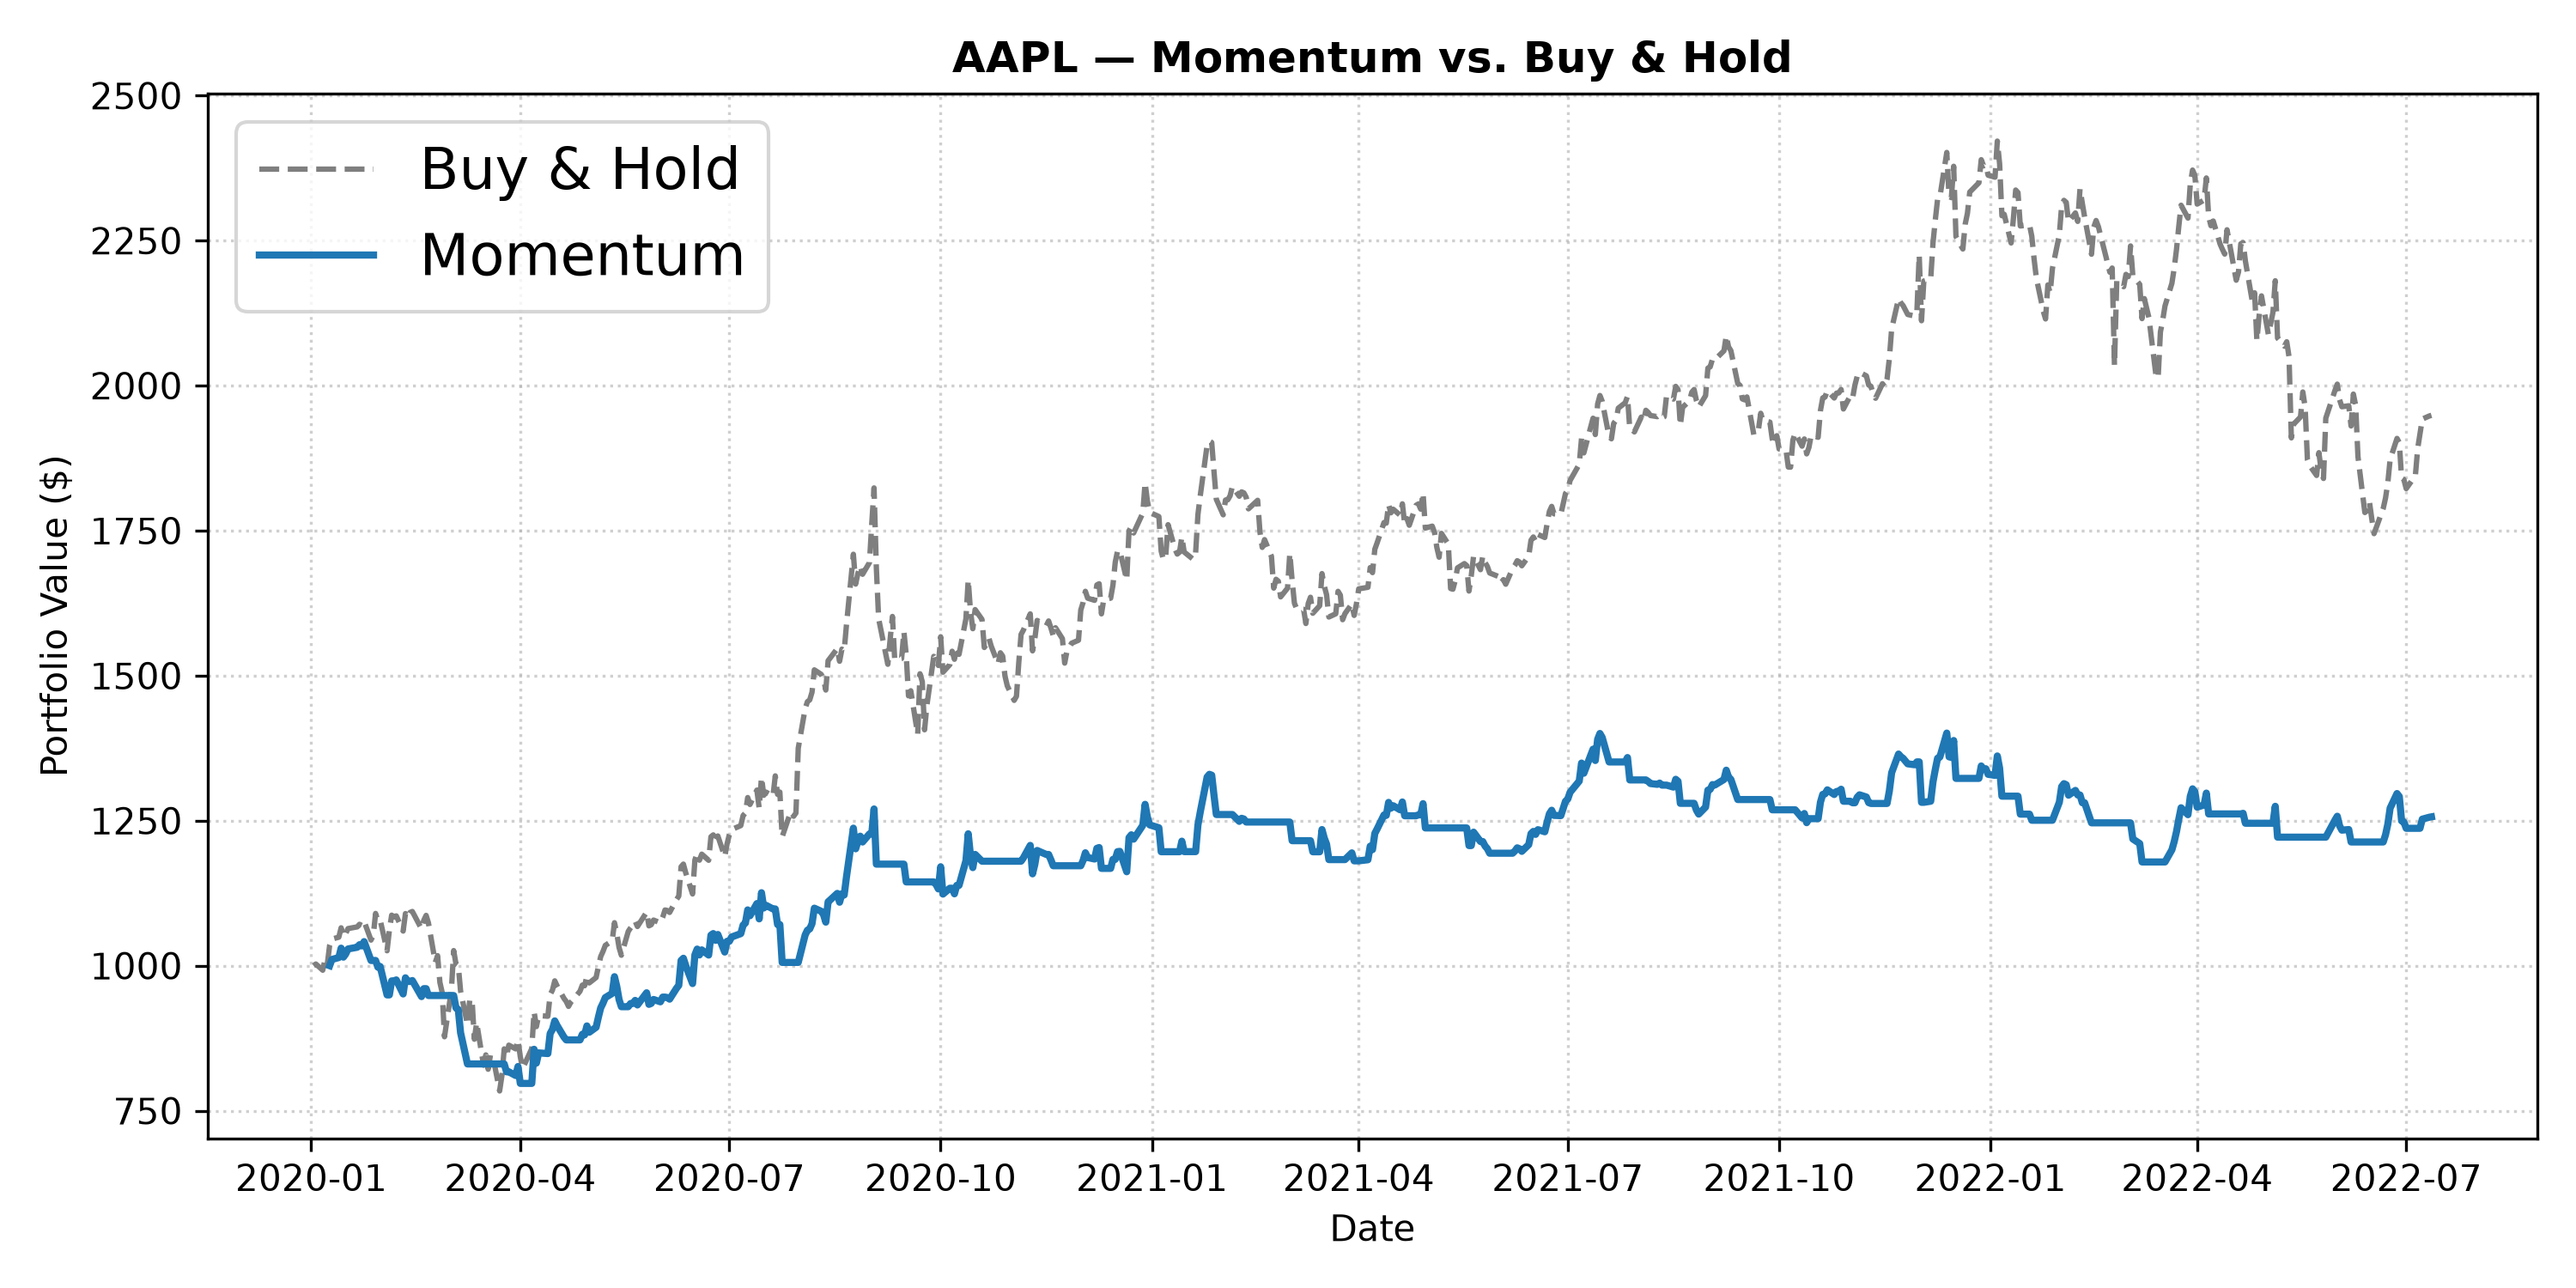
\includegraphics[width=0.85\textwidth]{../results/AAPL/AAPL_momentum_vs_bah.png}
    \caption{Performance comparison on AAPL (High-Volatility Growth Sector).}
    \label{fig:momentum_aapl}
\end{figure}

\begin{figure}[H]
    \centering
    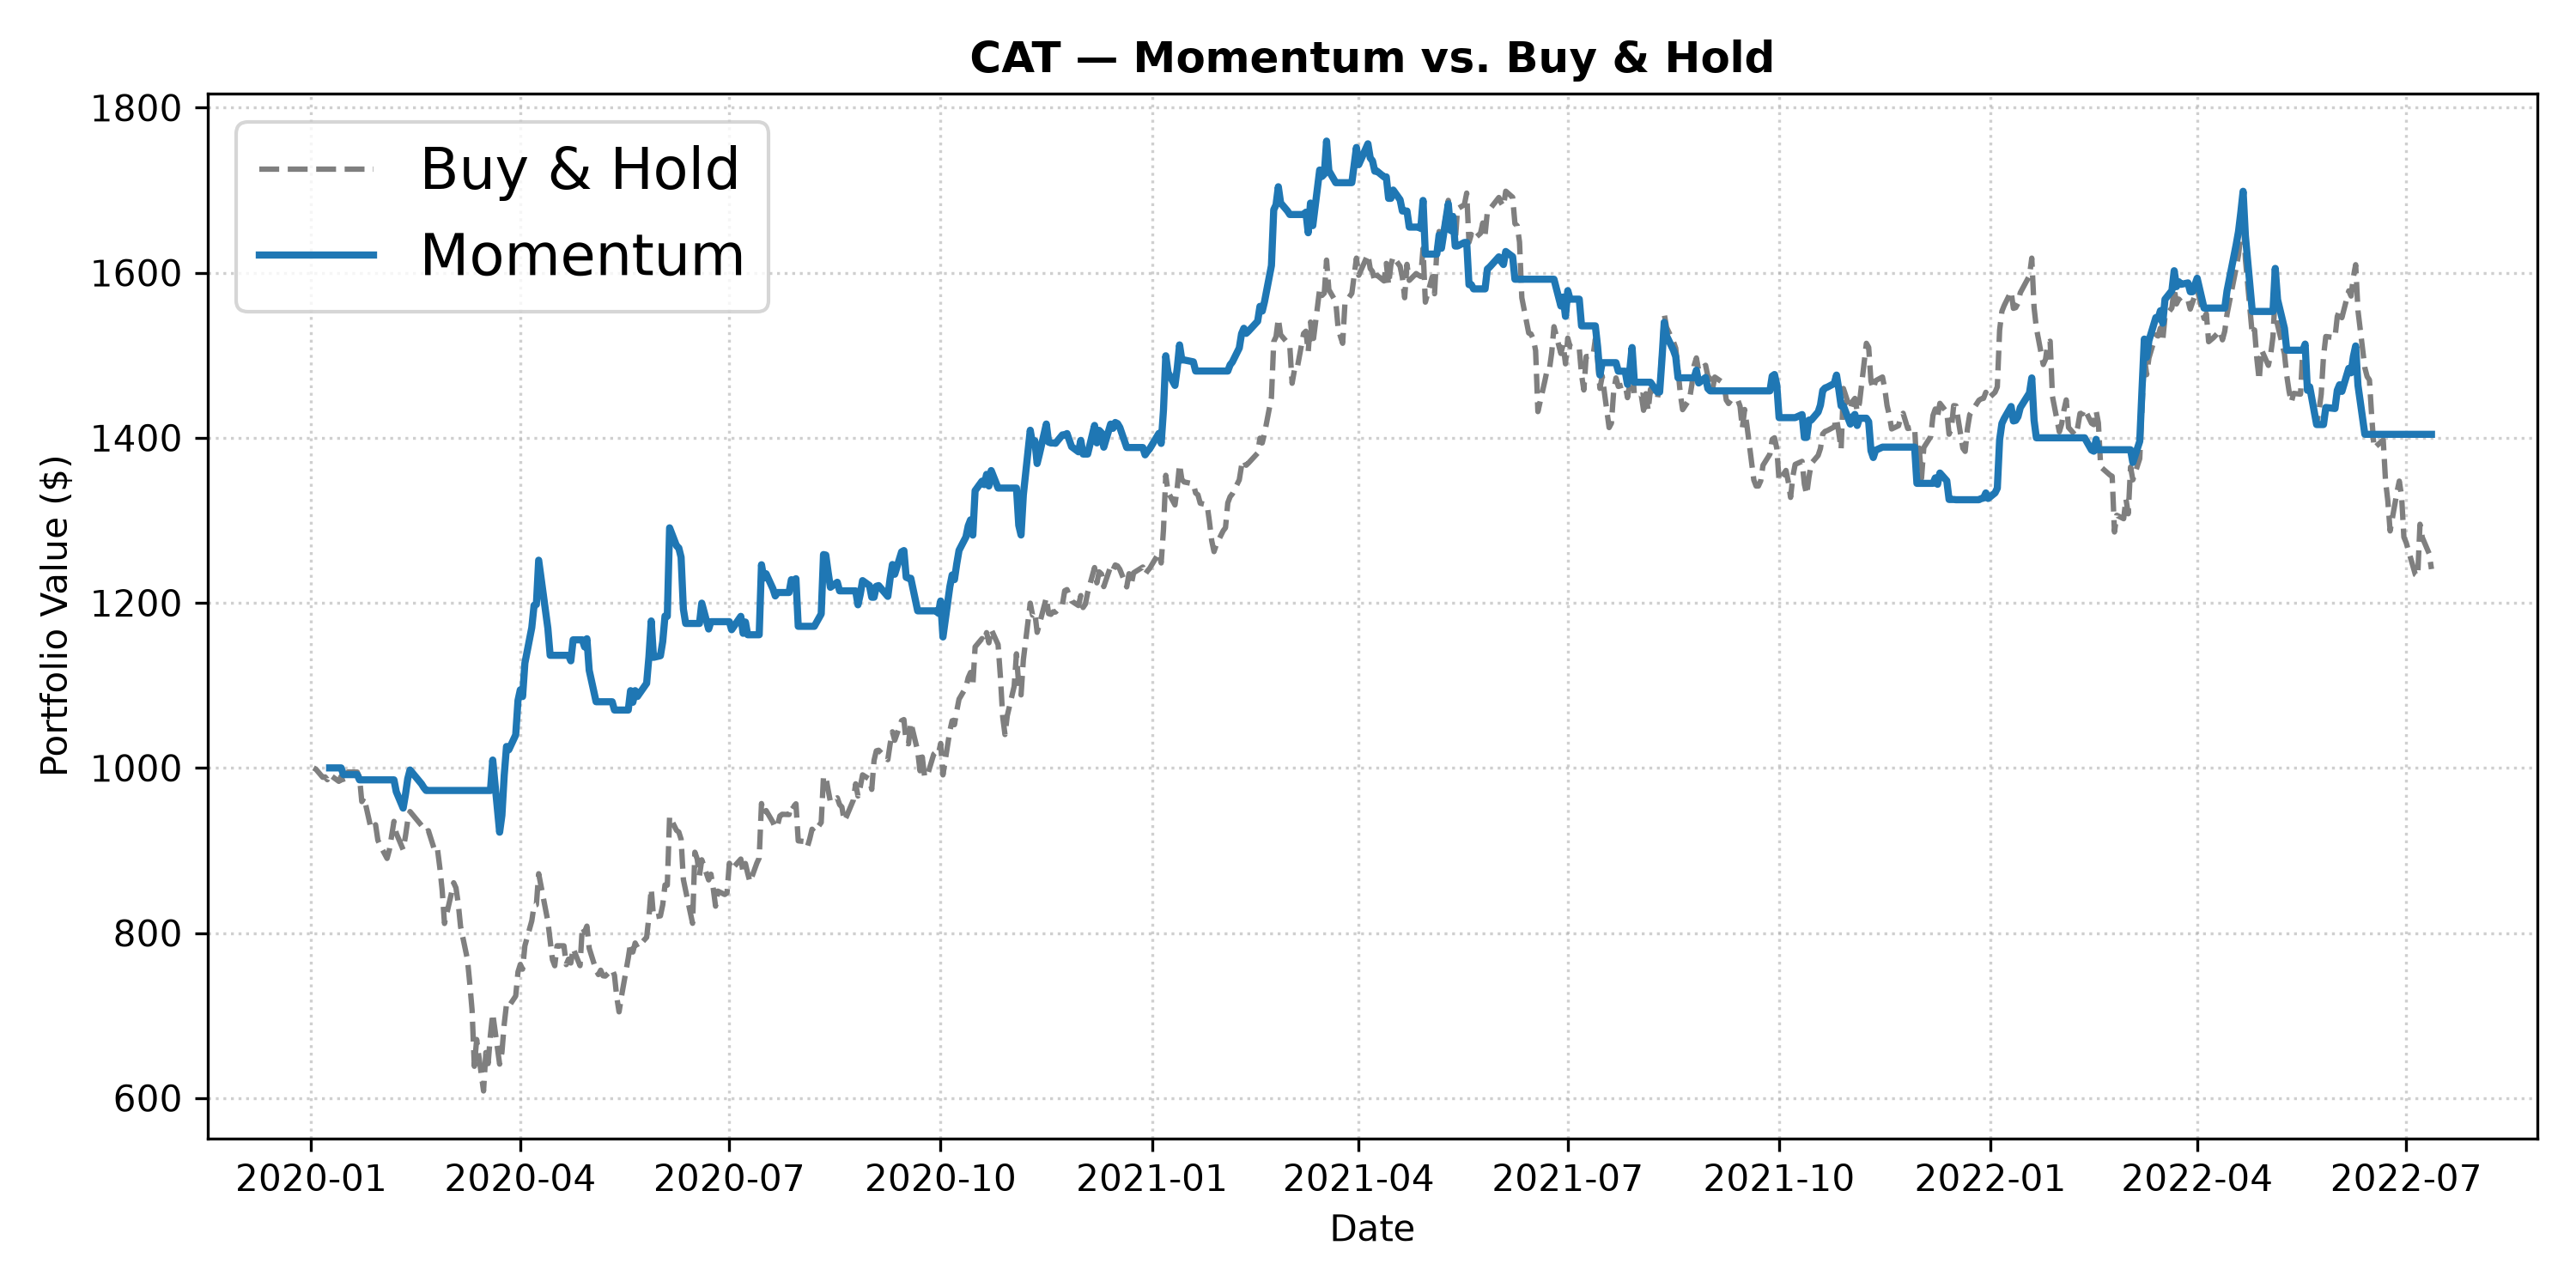
\includegraphics[width=0.85\textwidth]{../results/CAT/CAT_momentum_vs_bah.png}
    \caption{Performance comparison on CAT (Cyclical Industrial Sector).}
    \label{fig:momentum_cat}
\end{figure}

\begin{figure}[H]
    \centering
    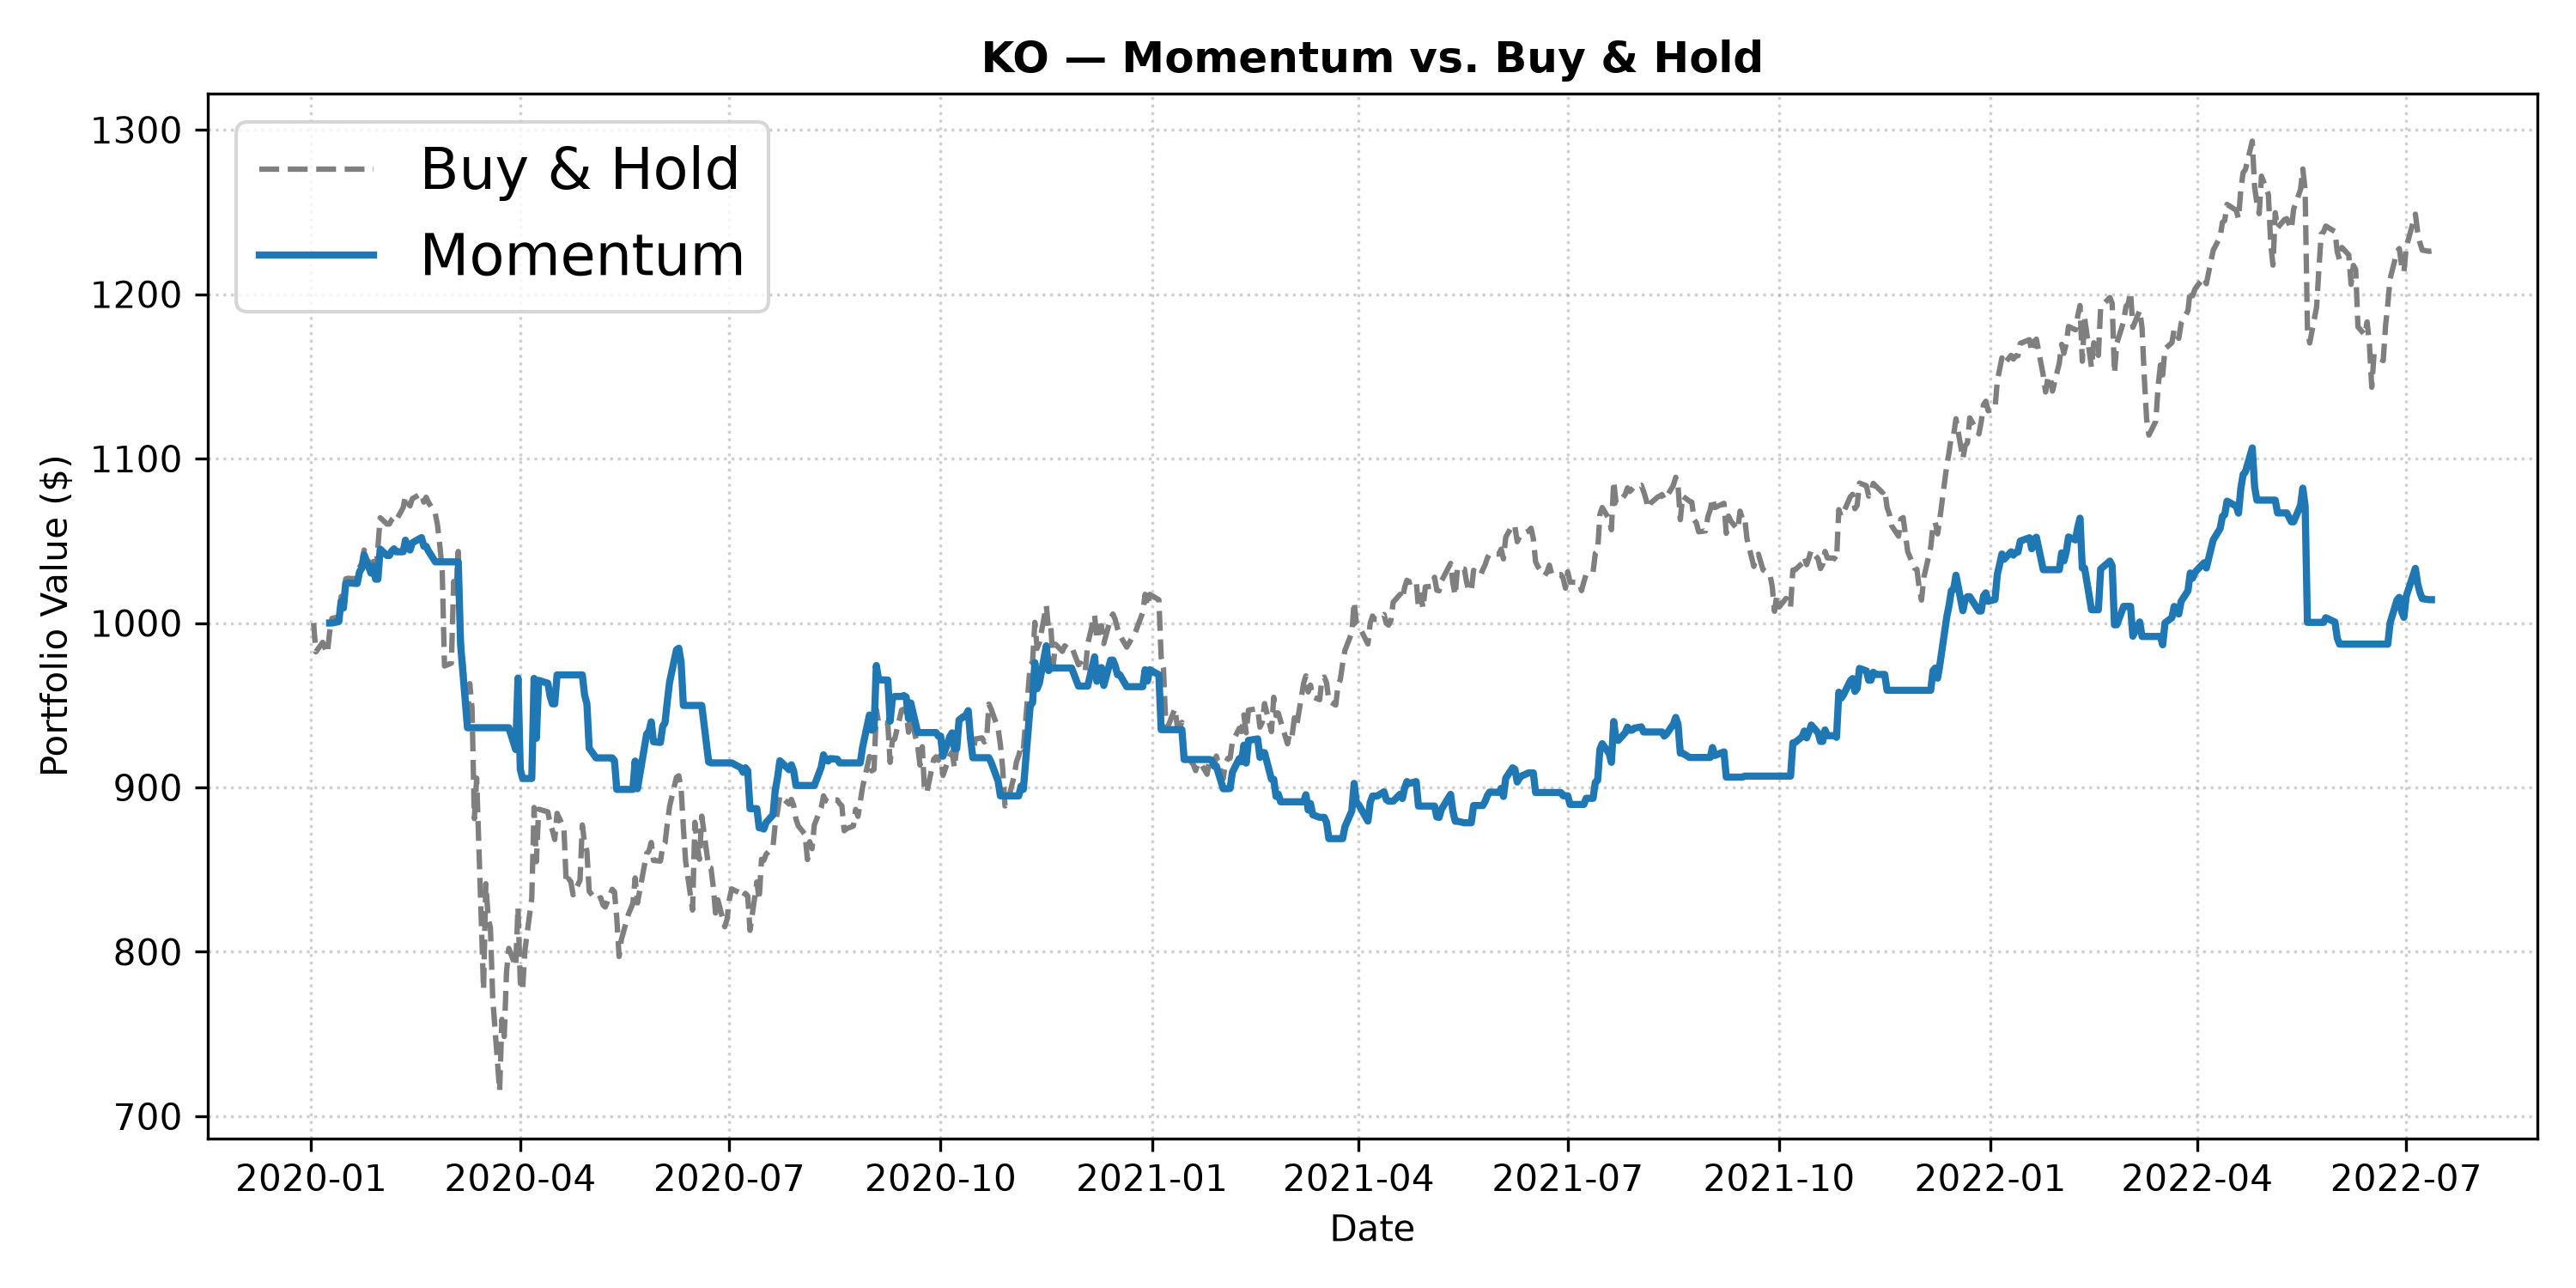
\includegraphics[width=0.85\textwidth]{../results/KO/KO_momentum_vs_bah.png}
    \caption{Performance comparison on KO (Defensive Consumer Staples Sector).}
    \label{fig:momentum_ko}
\end{figure}

\FloatBarrier

\subsection{Moving Average Performance}
The empirical backtest results for the Moving Average strategy demonstrate reduced portfolio turnover and drawdowns during prolonged structural shifts.

\begin{figure}[H]
    \centering
    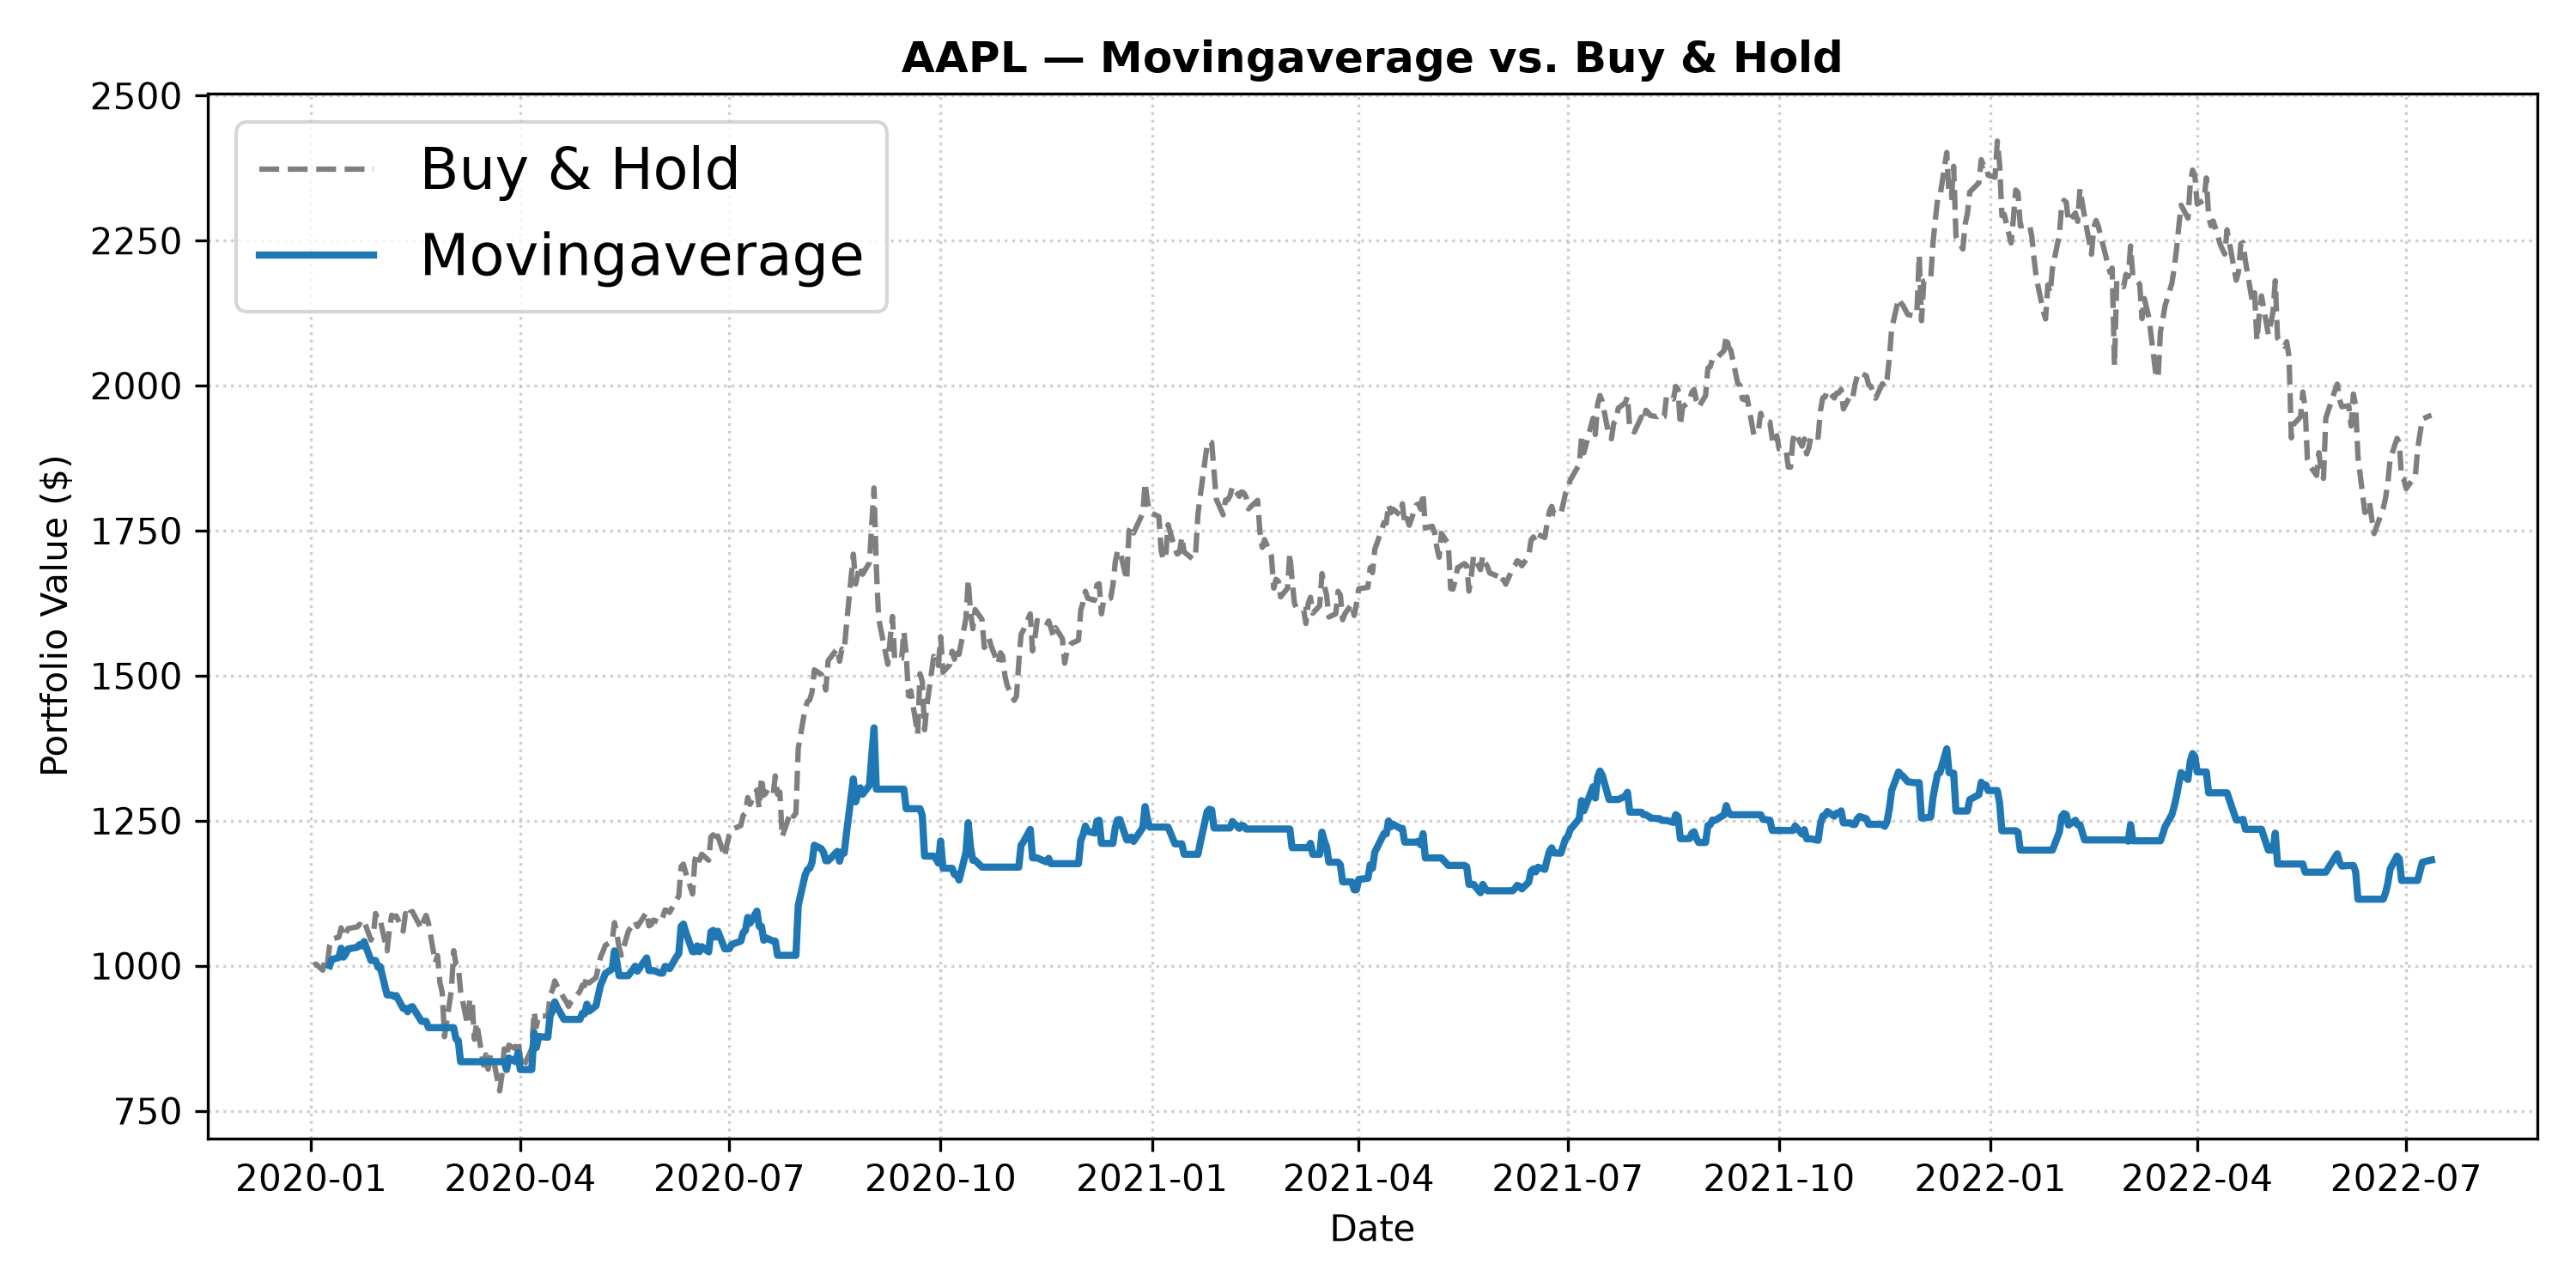
\includegraphics[width=0.85\textwidth]{../results/AAPL/AAPL_movingaverage_vs_bah.png}
    \caption{Performance comparison on AAPL (High-Volatility Growth Sector).}
    \label{fig:movingaverage_aapl}
\end{figure}

\begin{figure}[H]
    \centering
    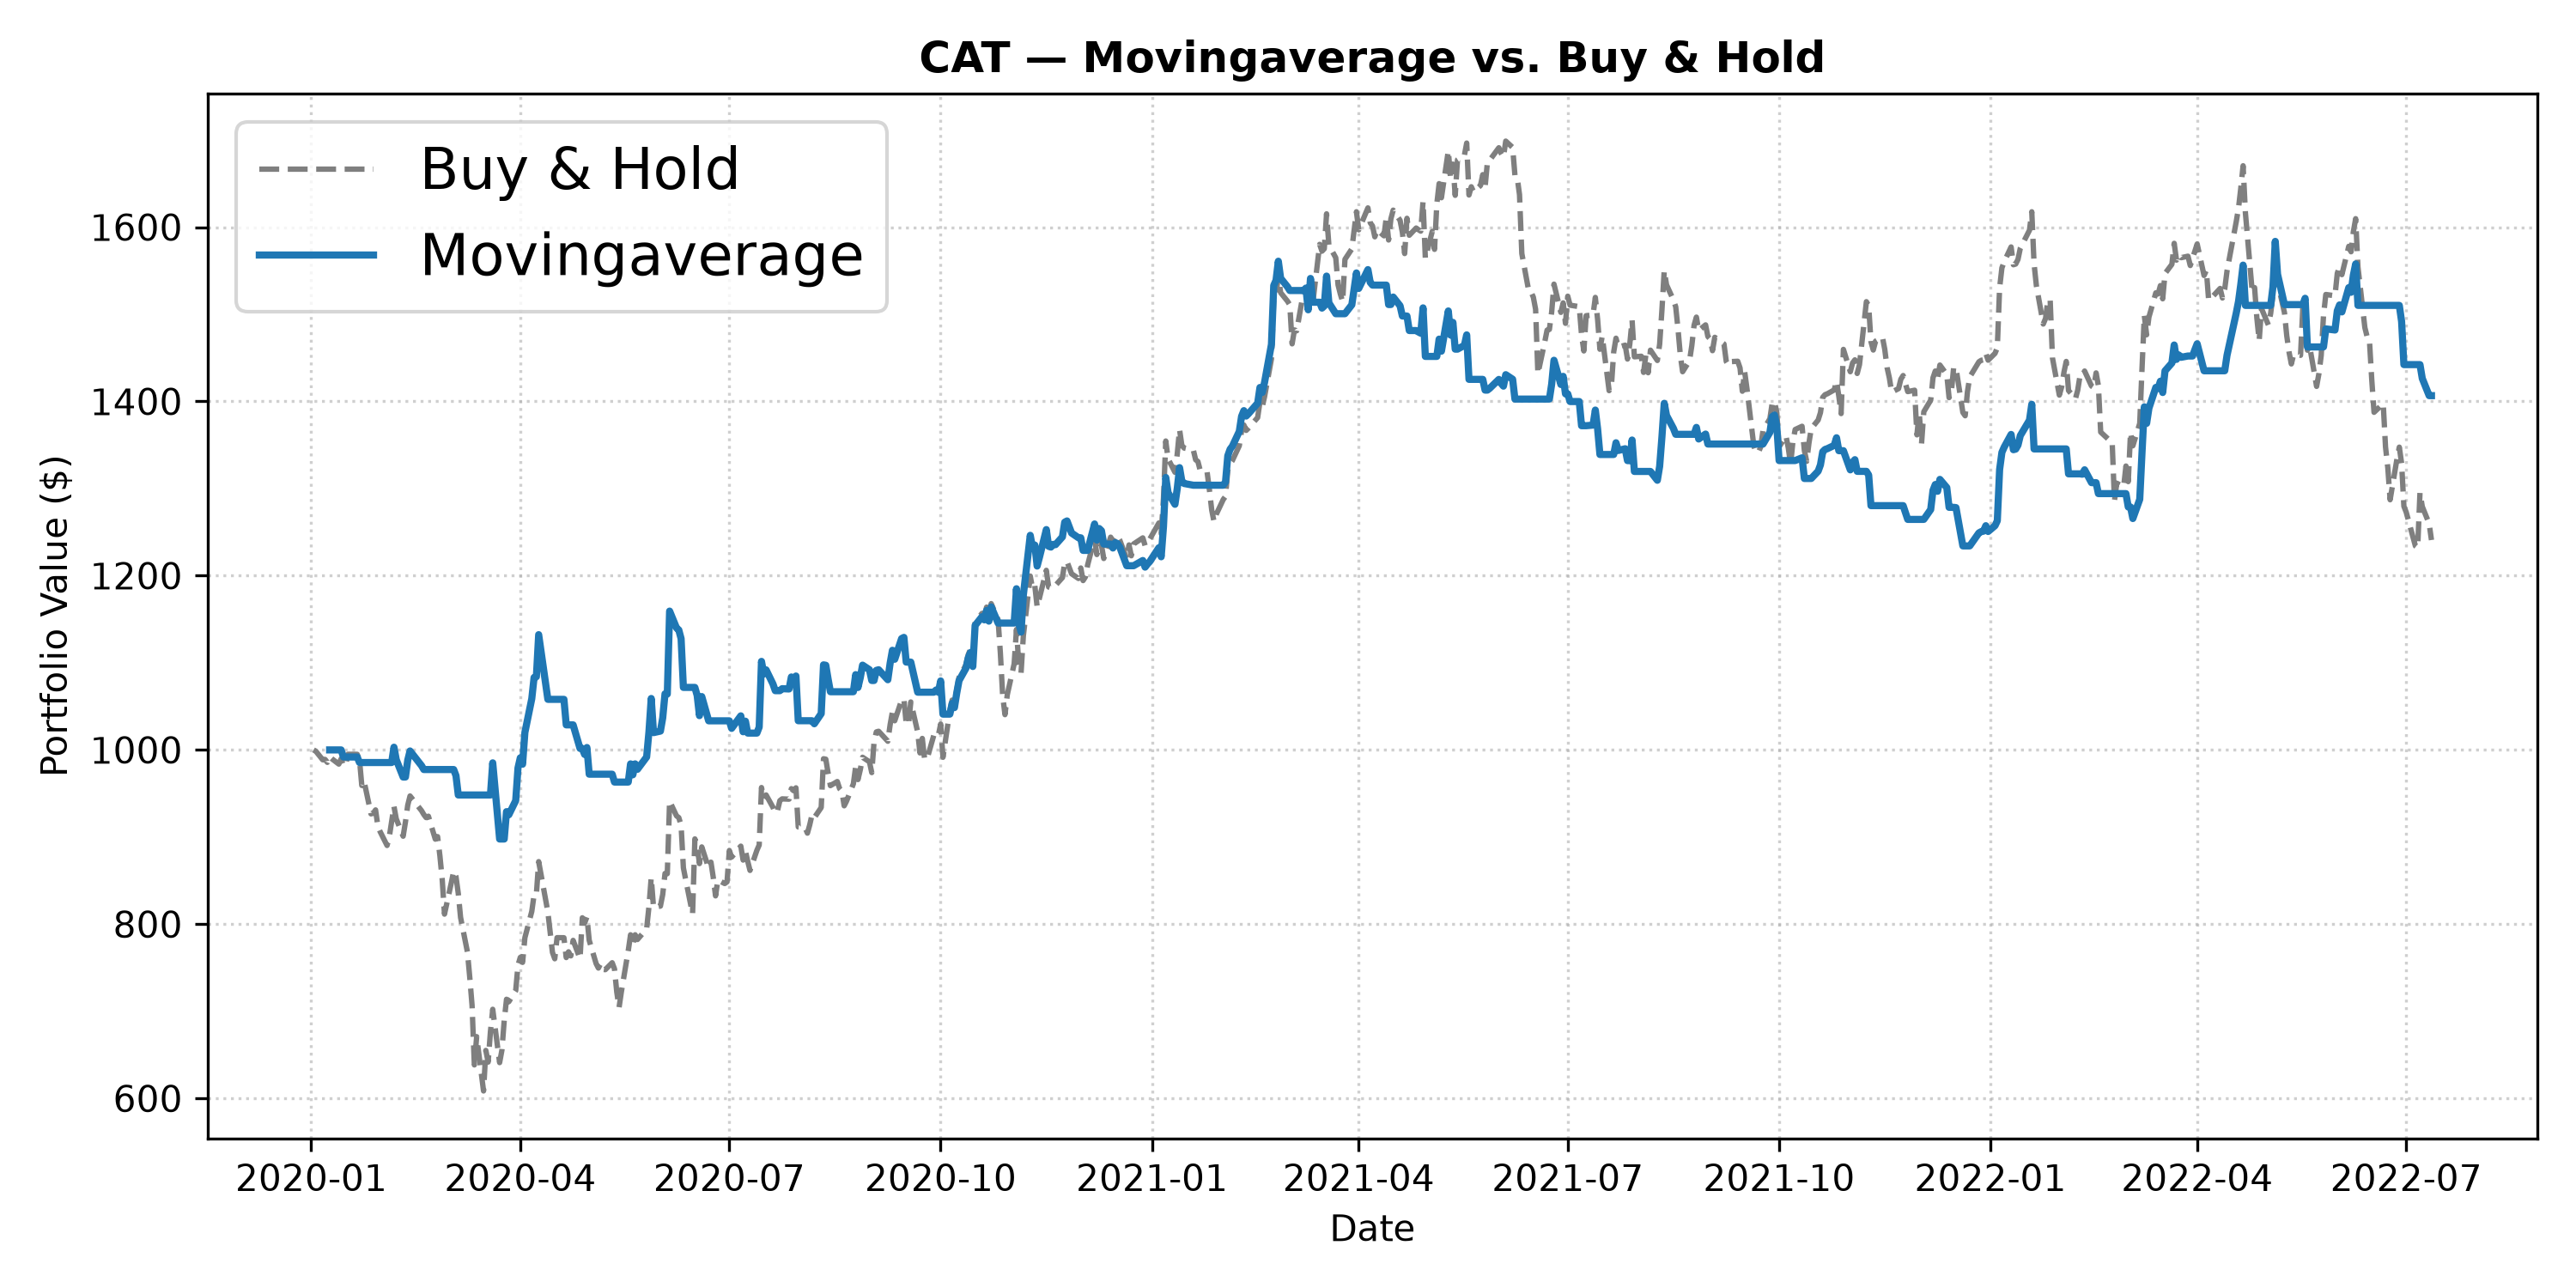
\includegraphics[width=0.85\textwidth]{../results/CAT/CAT_movingaverage_vs_bah.png}
    \caption{Performance comparison on CAT (Cyclical Industrial Sector).}
    \label{fig:movingaverage_cat}
\end{figure}

\begin{figure}[H]
    \centering
    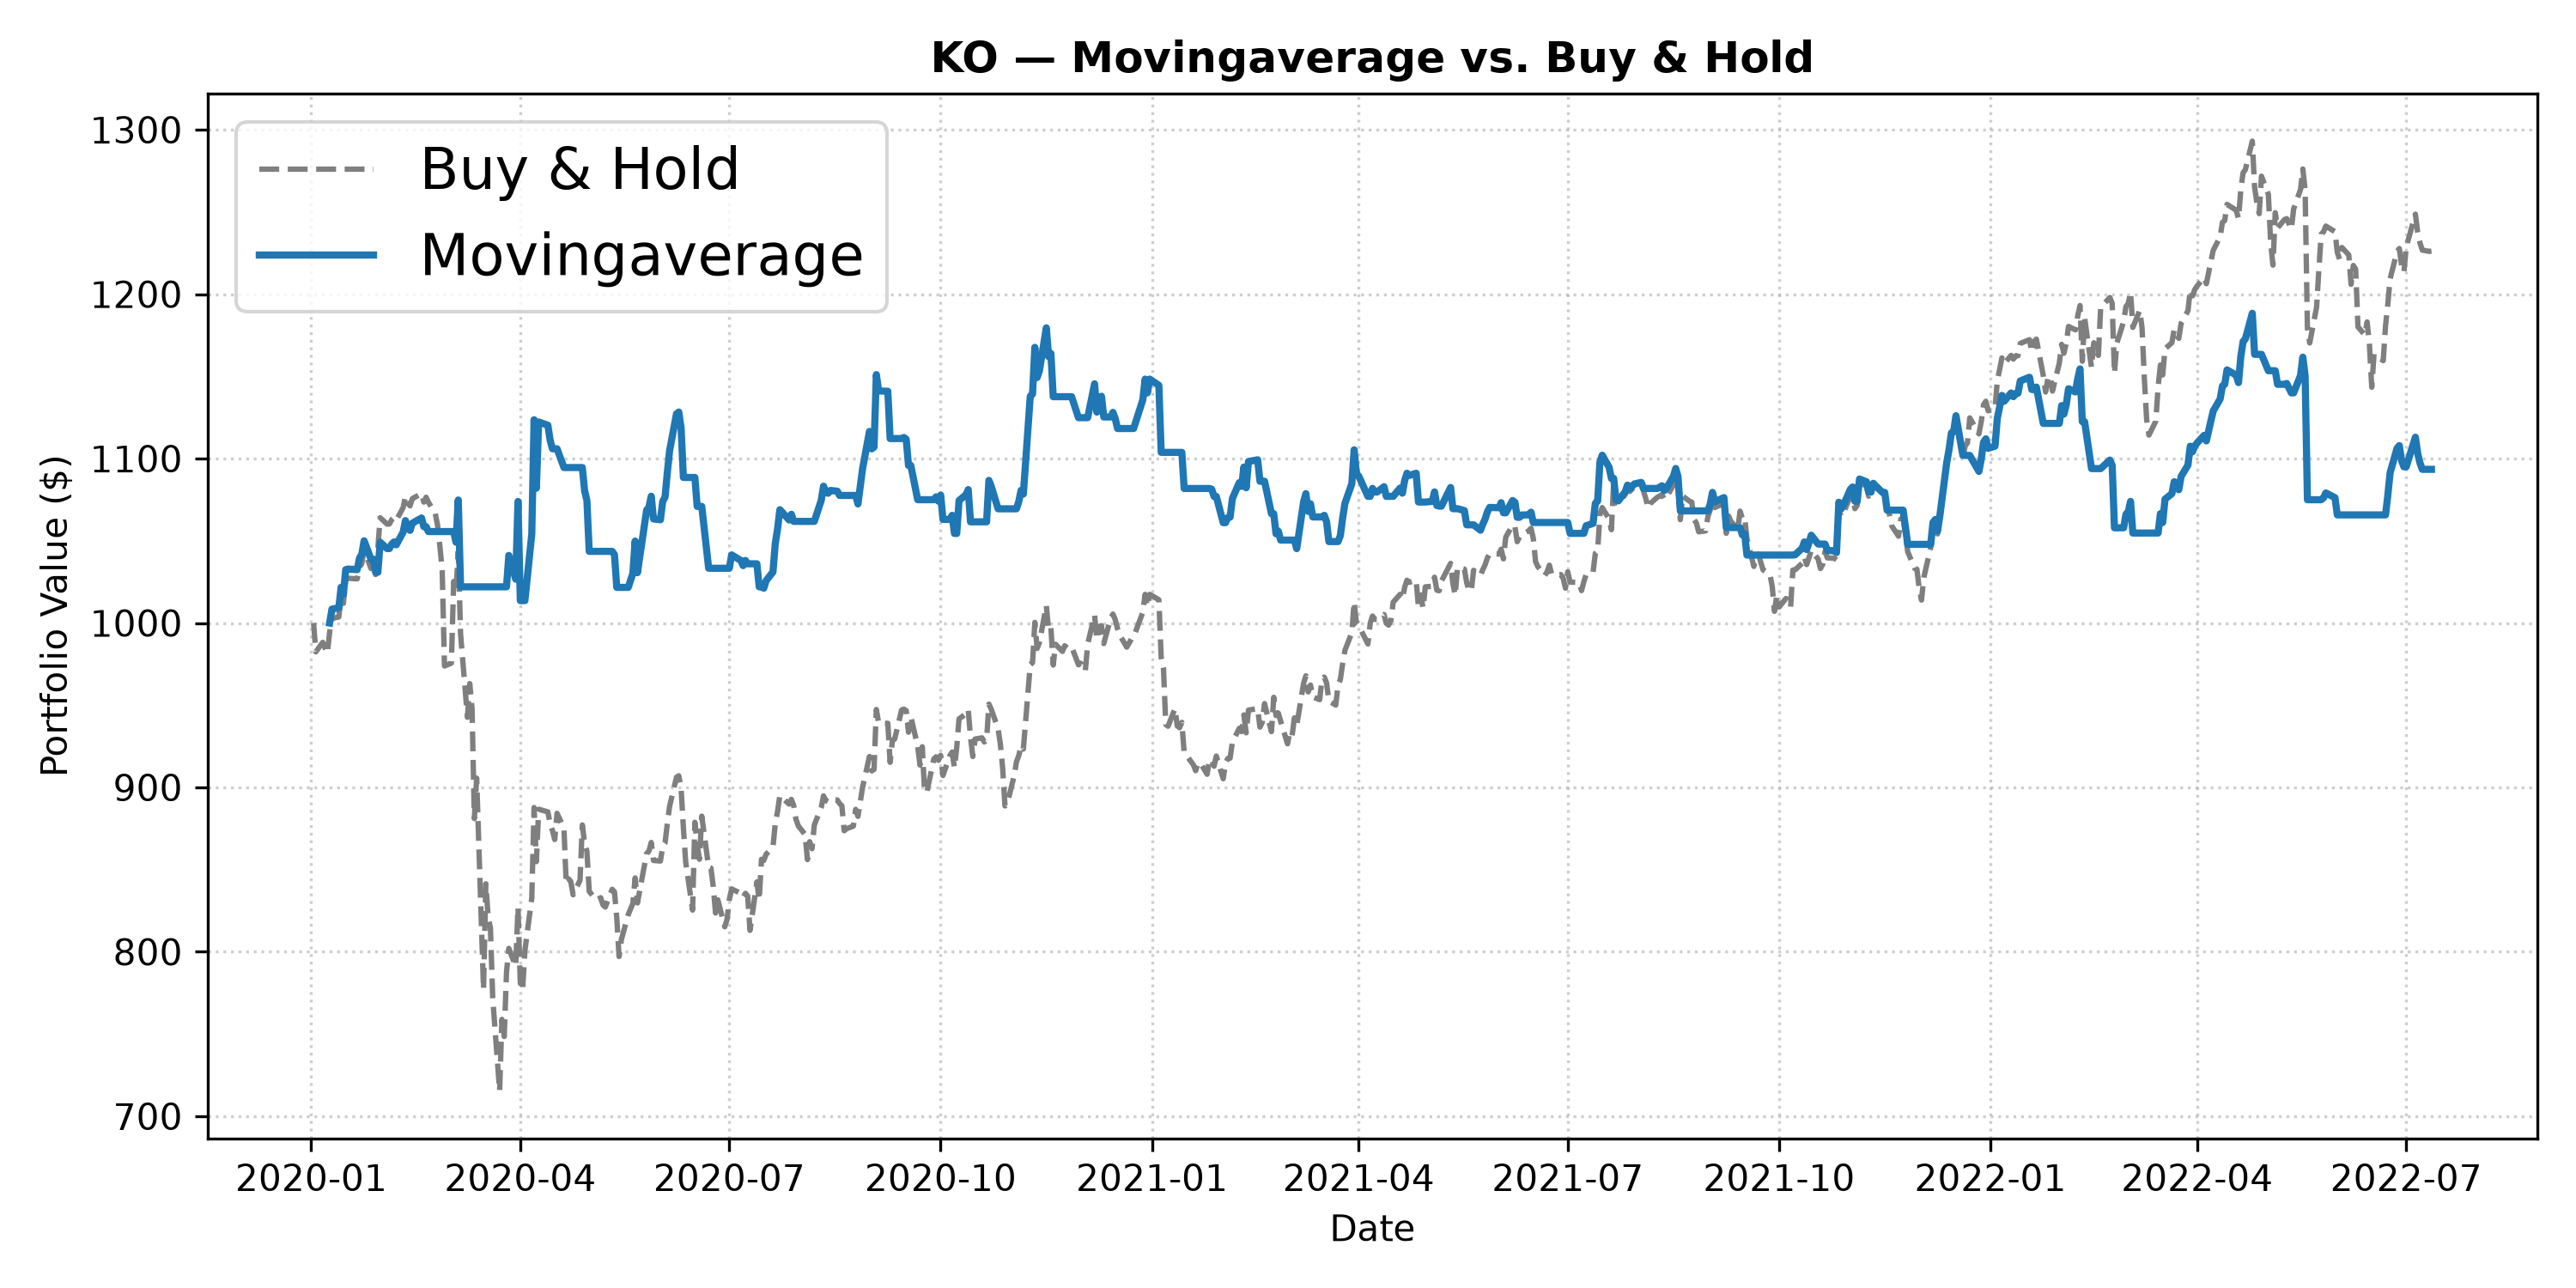
\includegraphics[width=0.85\textwidth]{../results/KO/KO_movingaverage_vs_bah.png}
    \caption{Performance comparison on KO (Defensive Consumer Staples Sector).}
    \label{fig:movingaverage_ko}
\end{figure}

\FloatBarrier

\subsection{KNN-Filtered Momentum Performance}
The KNN-filtered momentum strategy does not excel in any one of our tests. The strategy exhibits a relatively horizontal linear trend near its lower region.

\begin{figure}[H]
    \centering
    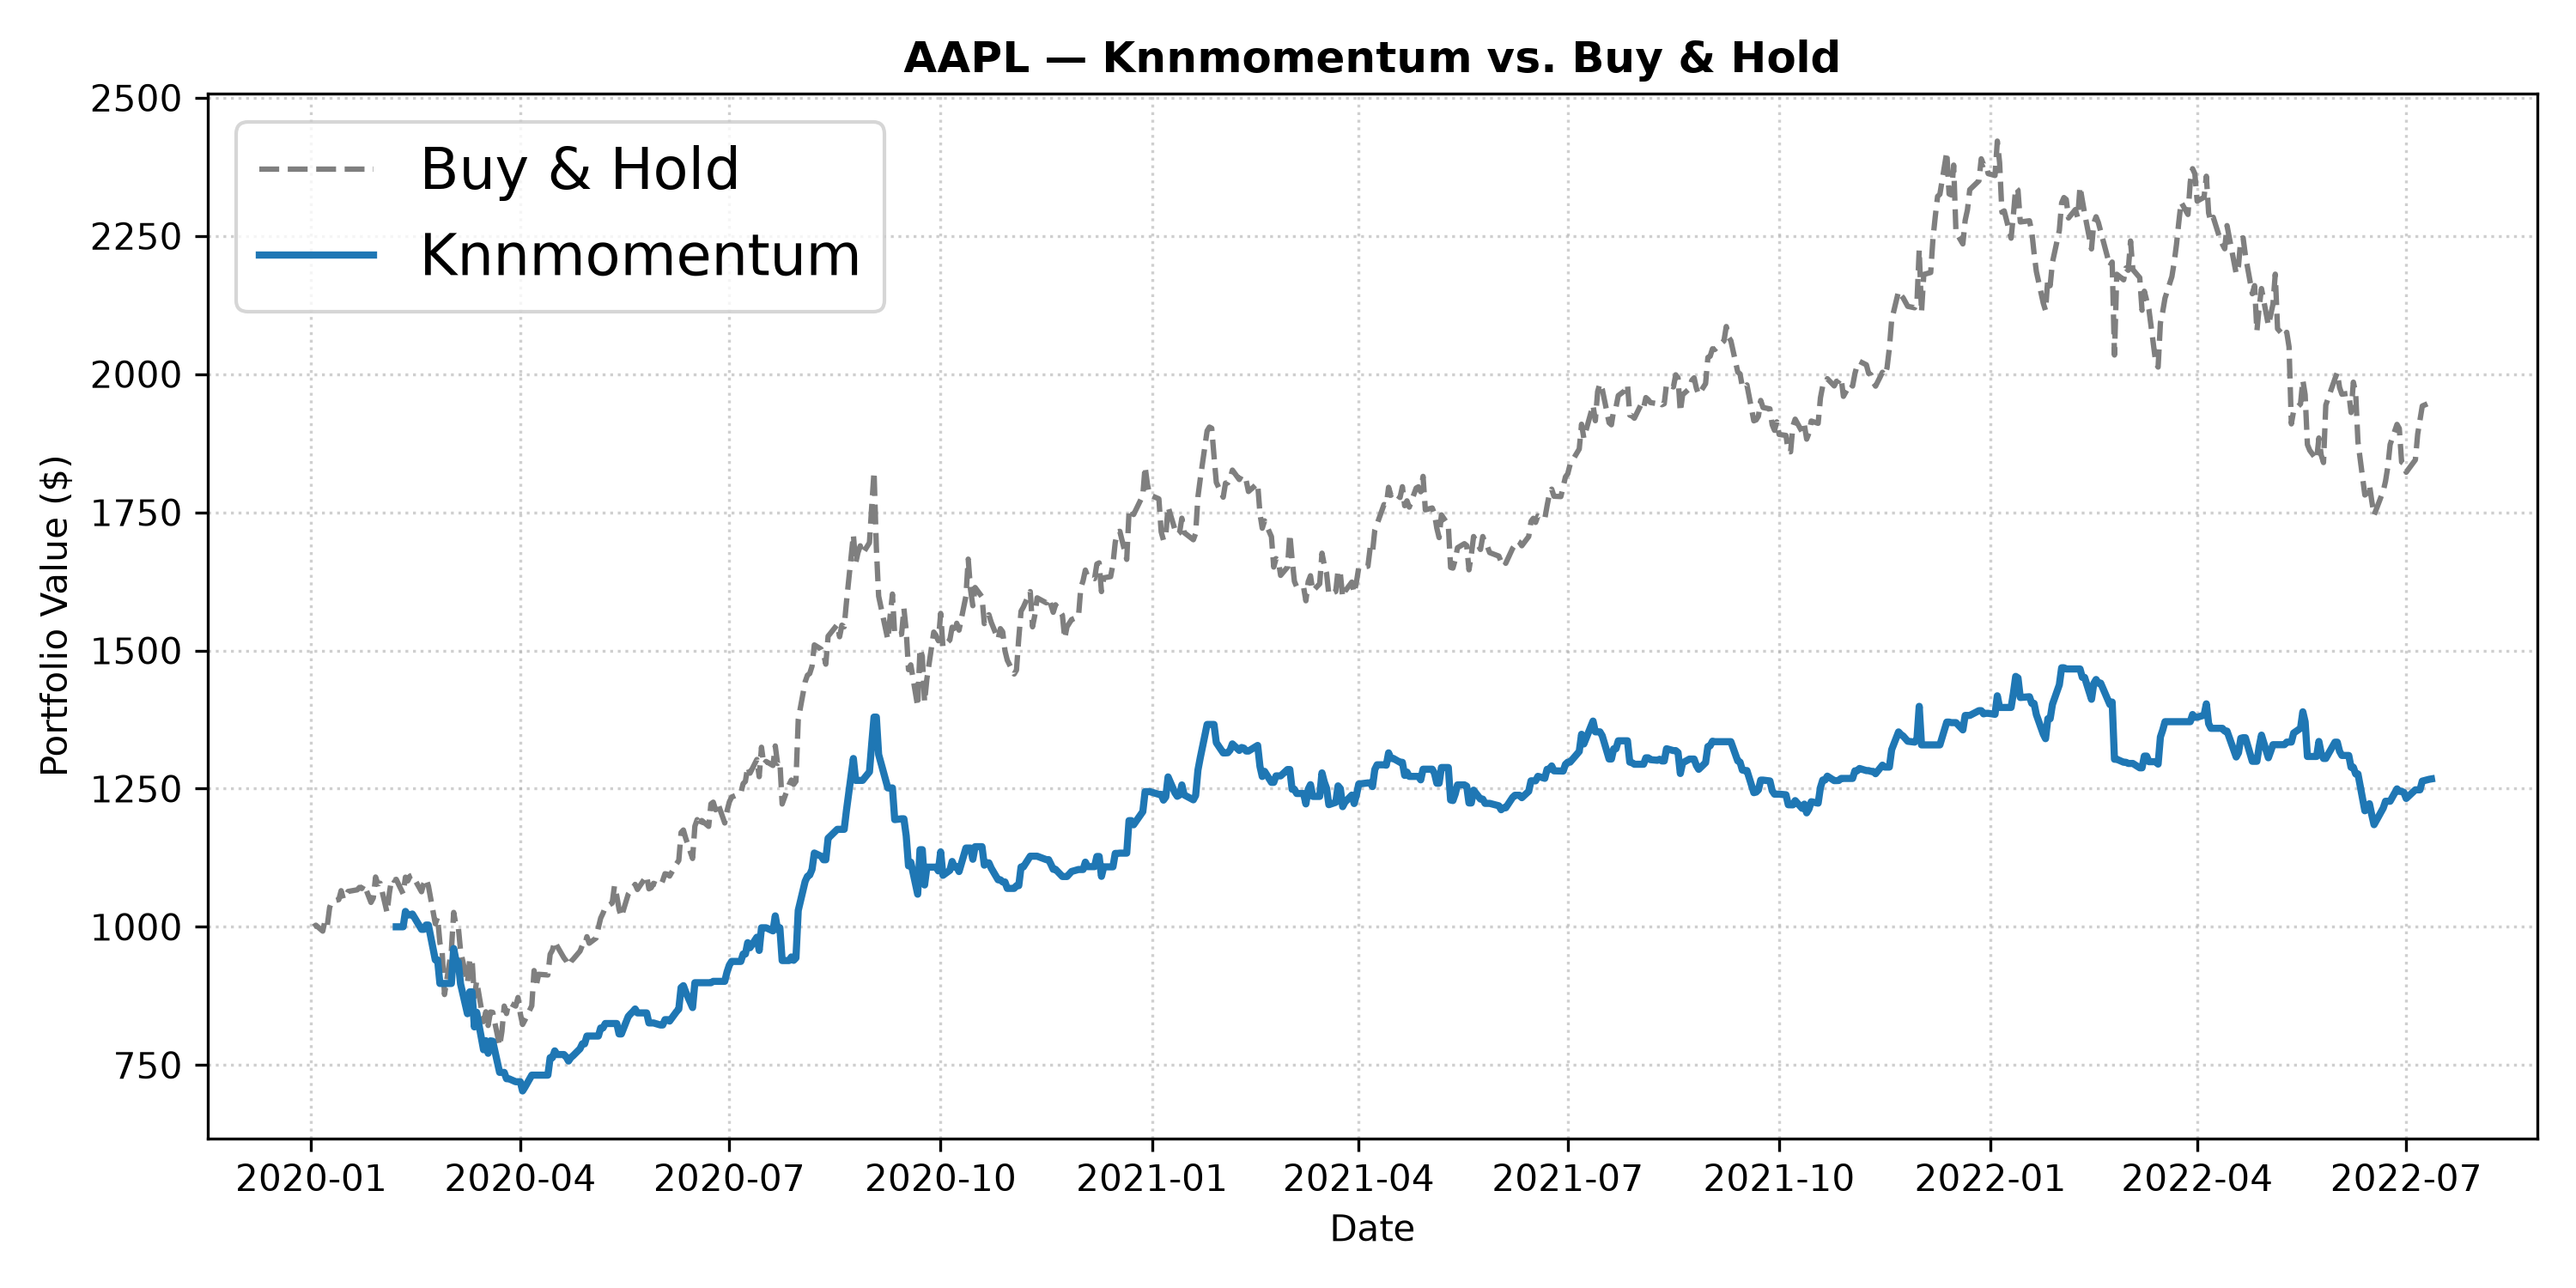
\includegraphics[width=0.85\textwidth]{../results/AAPL/AAPL_knnmomentum_vs_bah.png}
    \caption{Performance comparison on AAPL (High-Volatility Growth Sector).}
    \label{fig:knnmomentum_aapl}
\end{figure}

\begin{figure}[H]
    \centering
    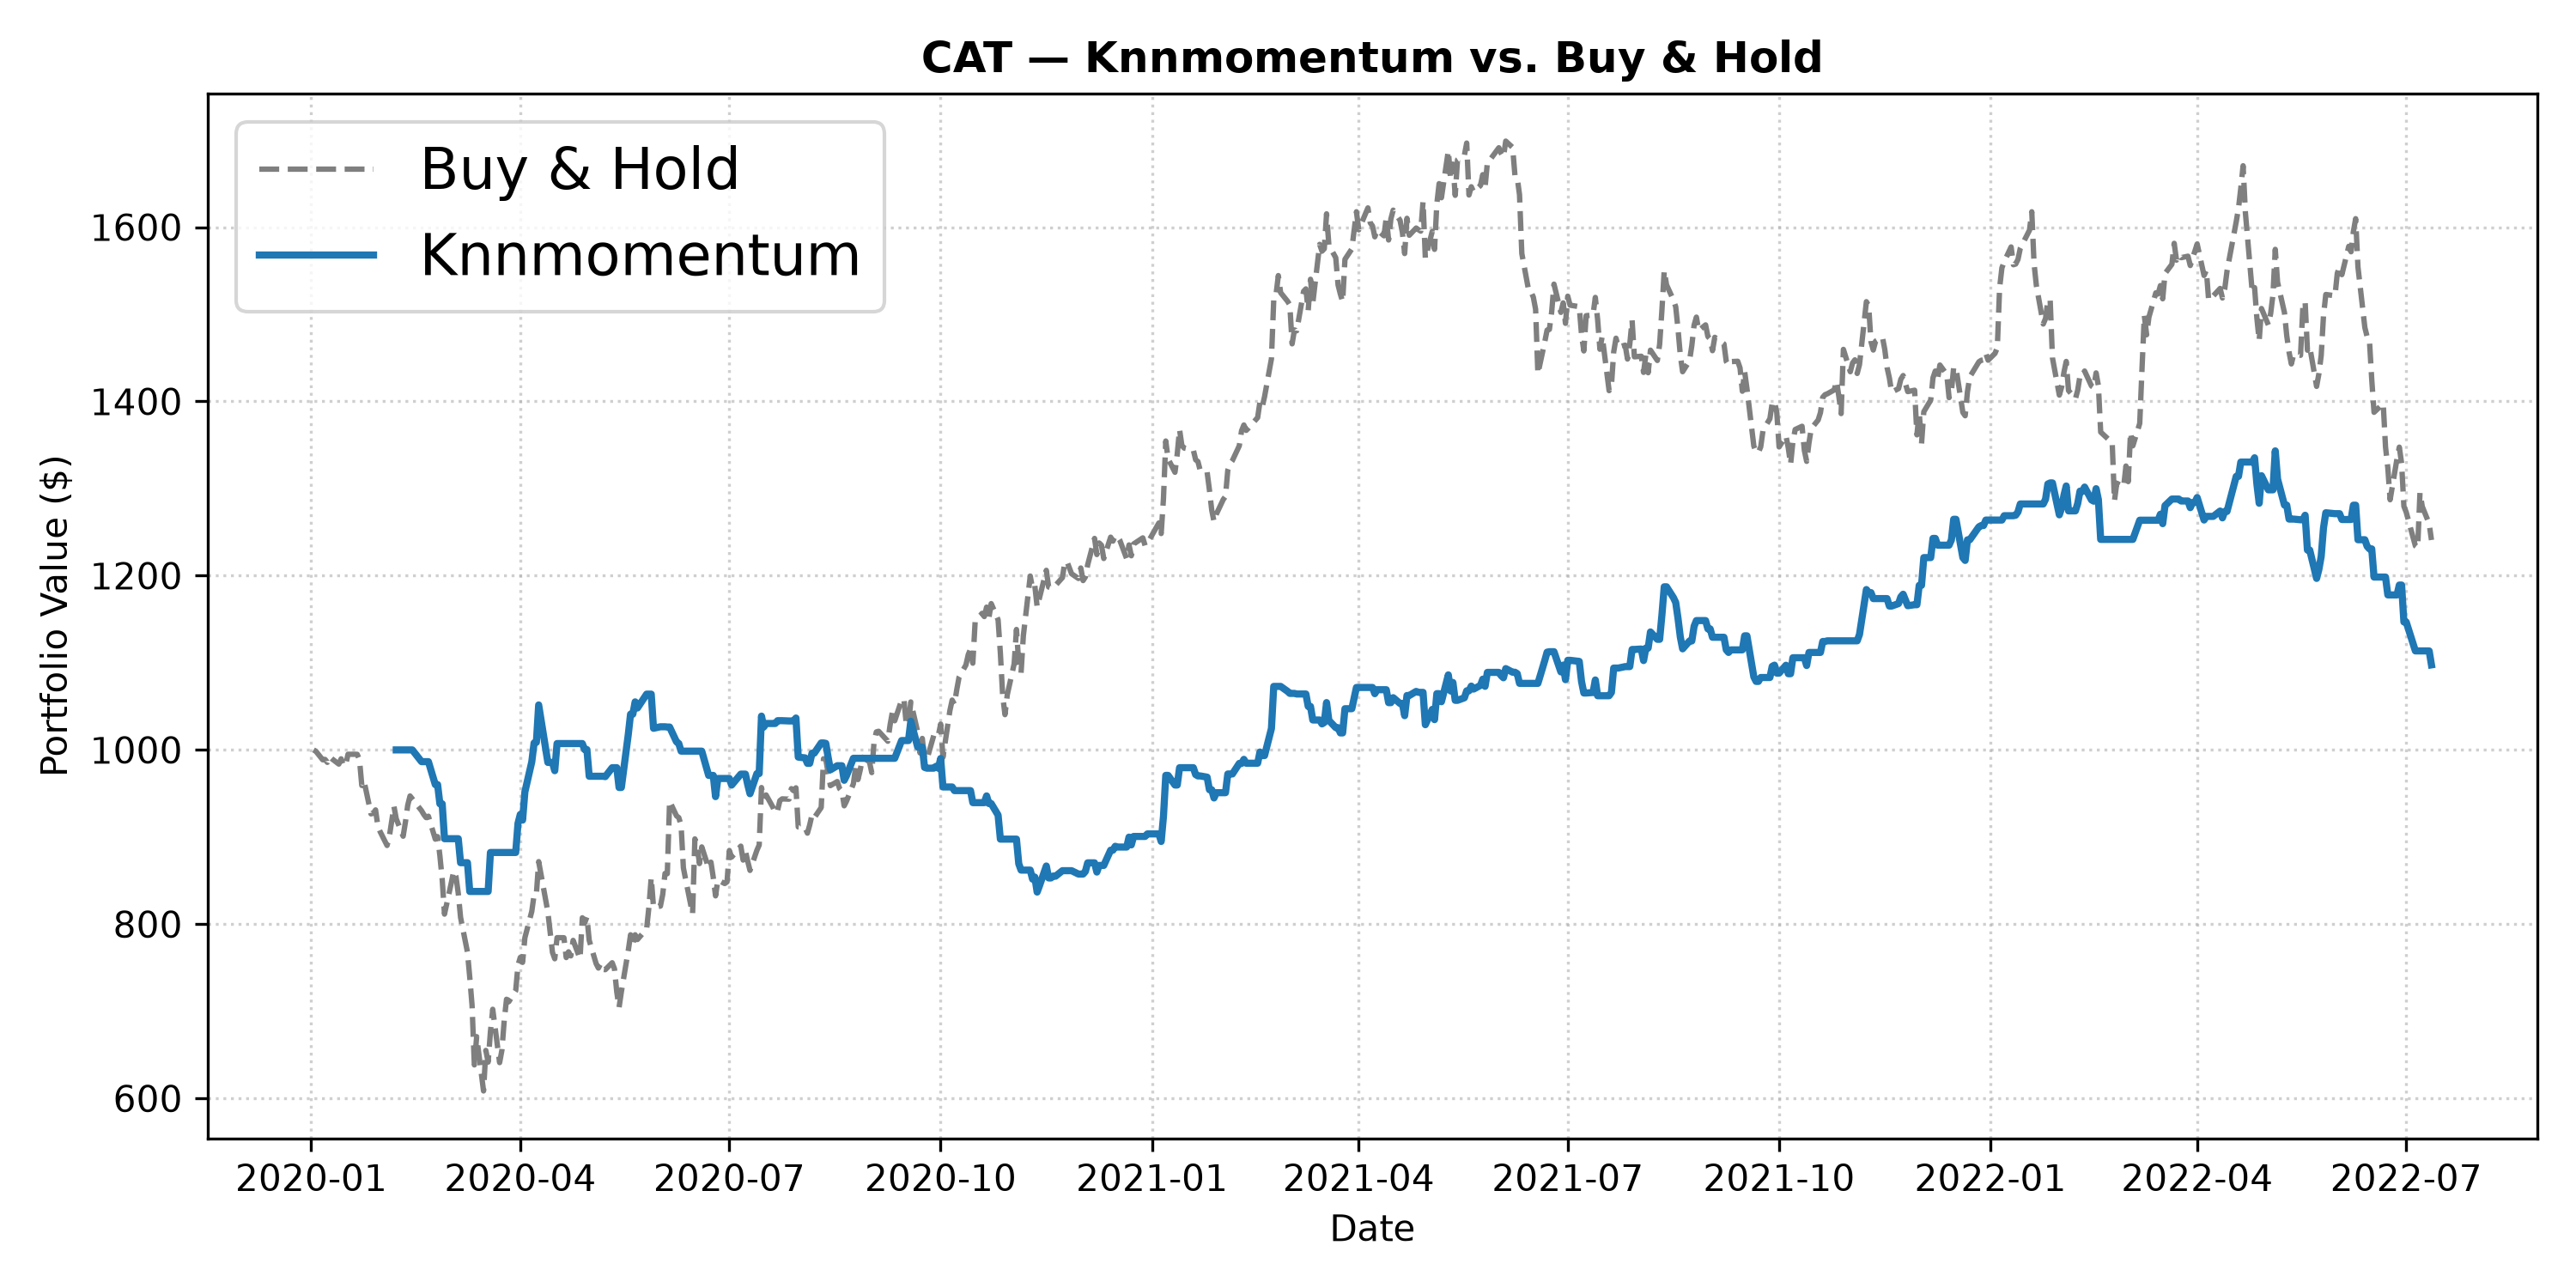
\includegraphics[width=0.85\textwidth]{../results/CAT/CAT_knnmomentum_vs_bah.png}
    \caption{Performance comparison on CAT (Cyclical Industrial Sector).}
    \label{fig:knnmomentum_cat}
\end{figure}

\begin{figure}[H]
    \centering
    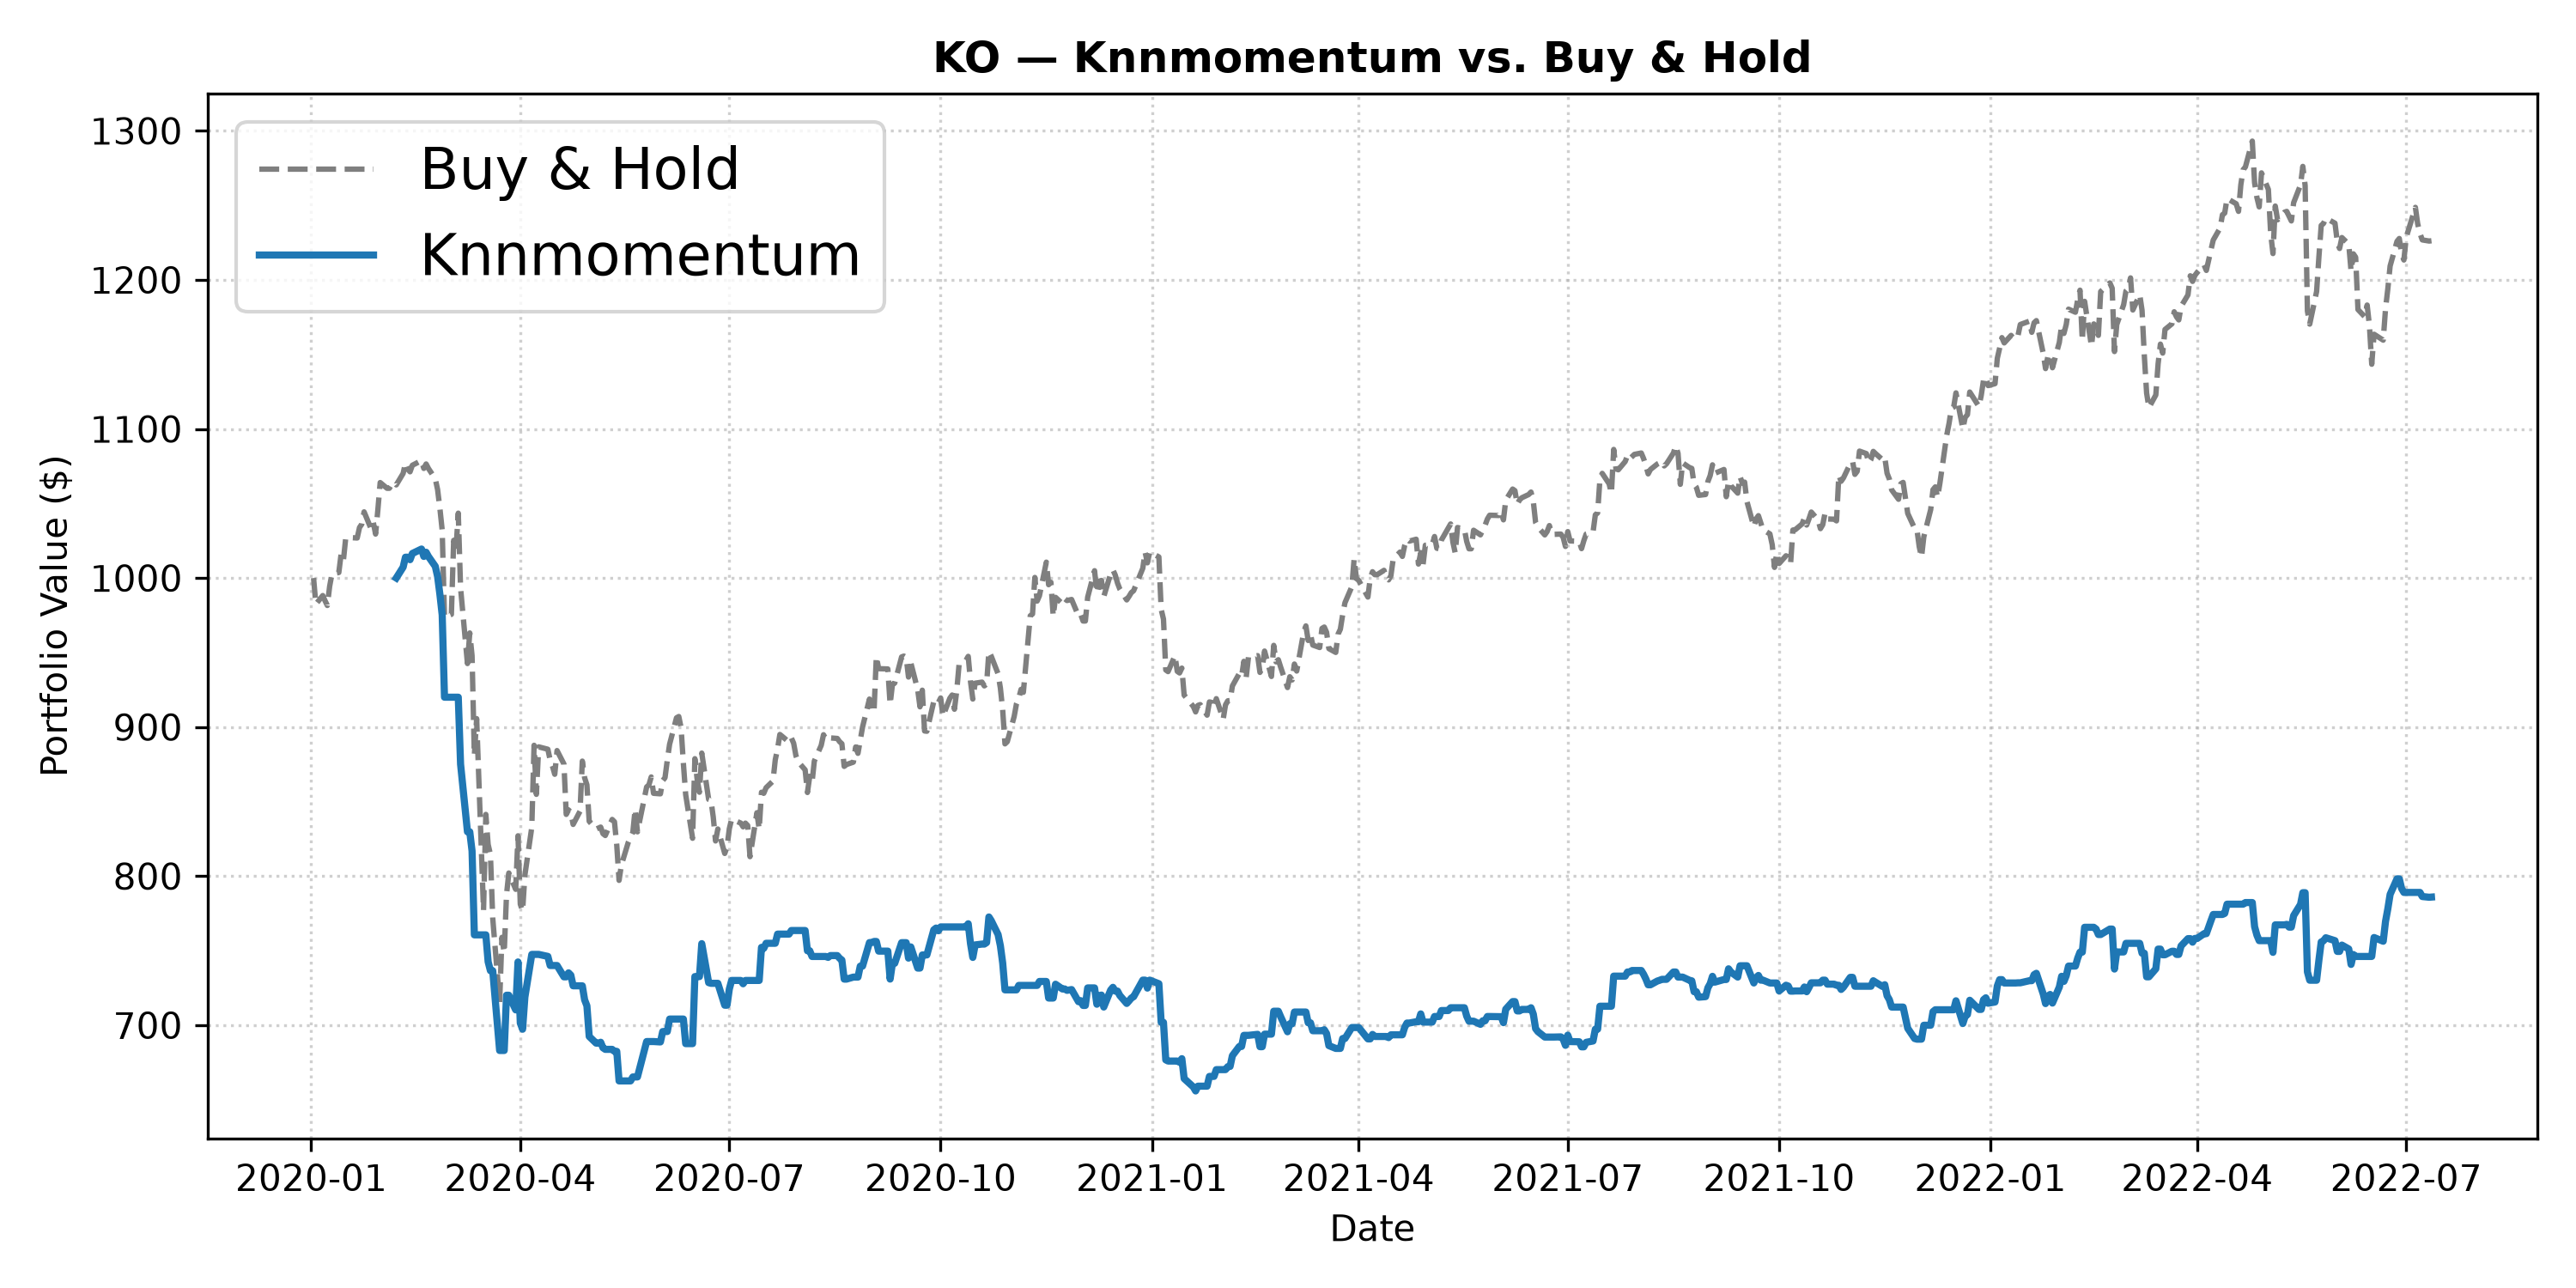
\includegraphics[width=0.85\textwidth]{../results/KO/KO_knnmomentum_vs_bah.png}
    \caption{Performance comparison on KO (Defensive Consumer Staples Sector).}
    \label{fig:knnmomentum_ko}
\end{figure}

\subsection{Standard Deviation Moving Average Mean Reversion Performance}

The standard deviation moving average mean reversion strategy severely underperforms the buy-and-hold baseline across all tested equities. By waiting for rare, extreme statistical deviations to trigger entries and exits, the strategy spends prolonged periods sitting in cash, thereby missing the multi-year compound growth of long-term upward trends.

\begin{figure}[H]
    \centering
    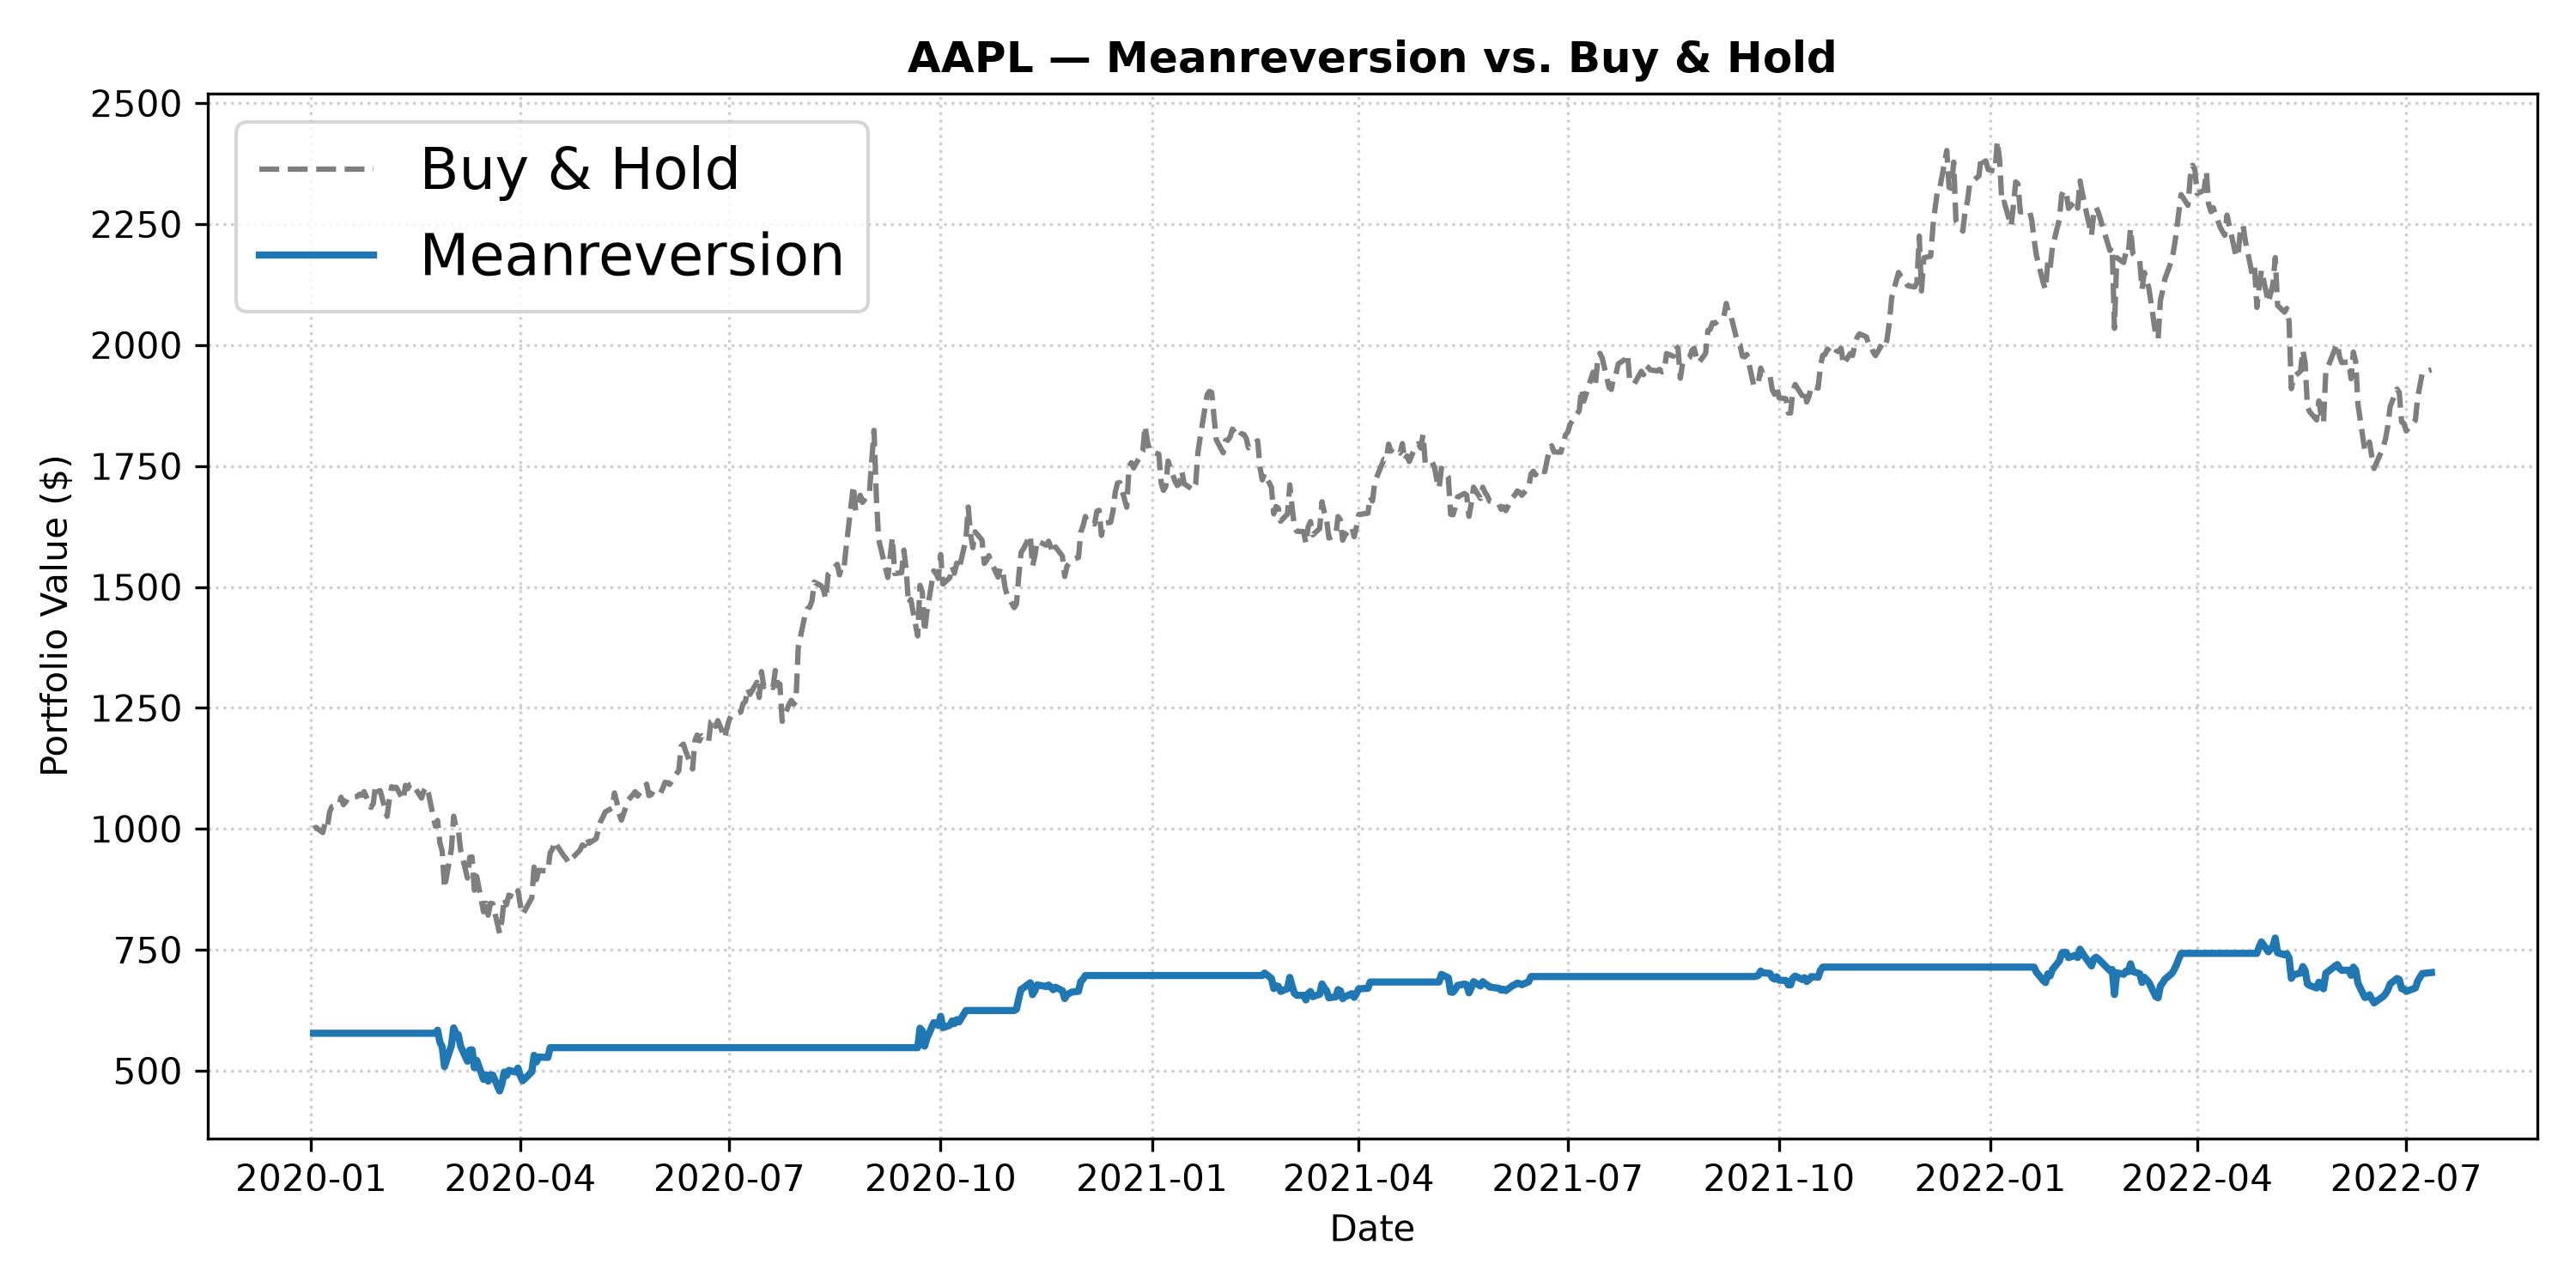
\includegraphics[width=0.85\textwidth]{../results/AAPL/AAPL_meanreversion_vs_bah.png}
    \caption{Performance comparison on AAPL (High-Volatility Growth Sector).}
    \label{fig:meanreversion_aapl}
\end{figure}

\begin{figure}[H]
    \centering
    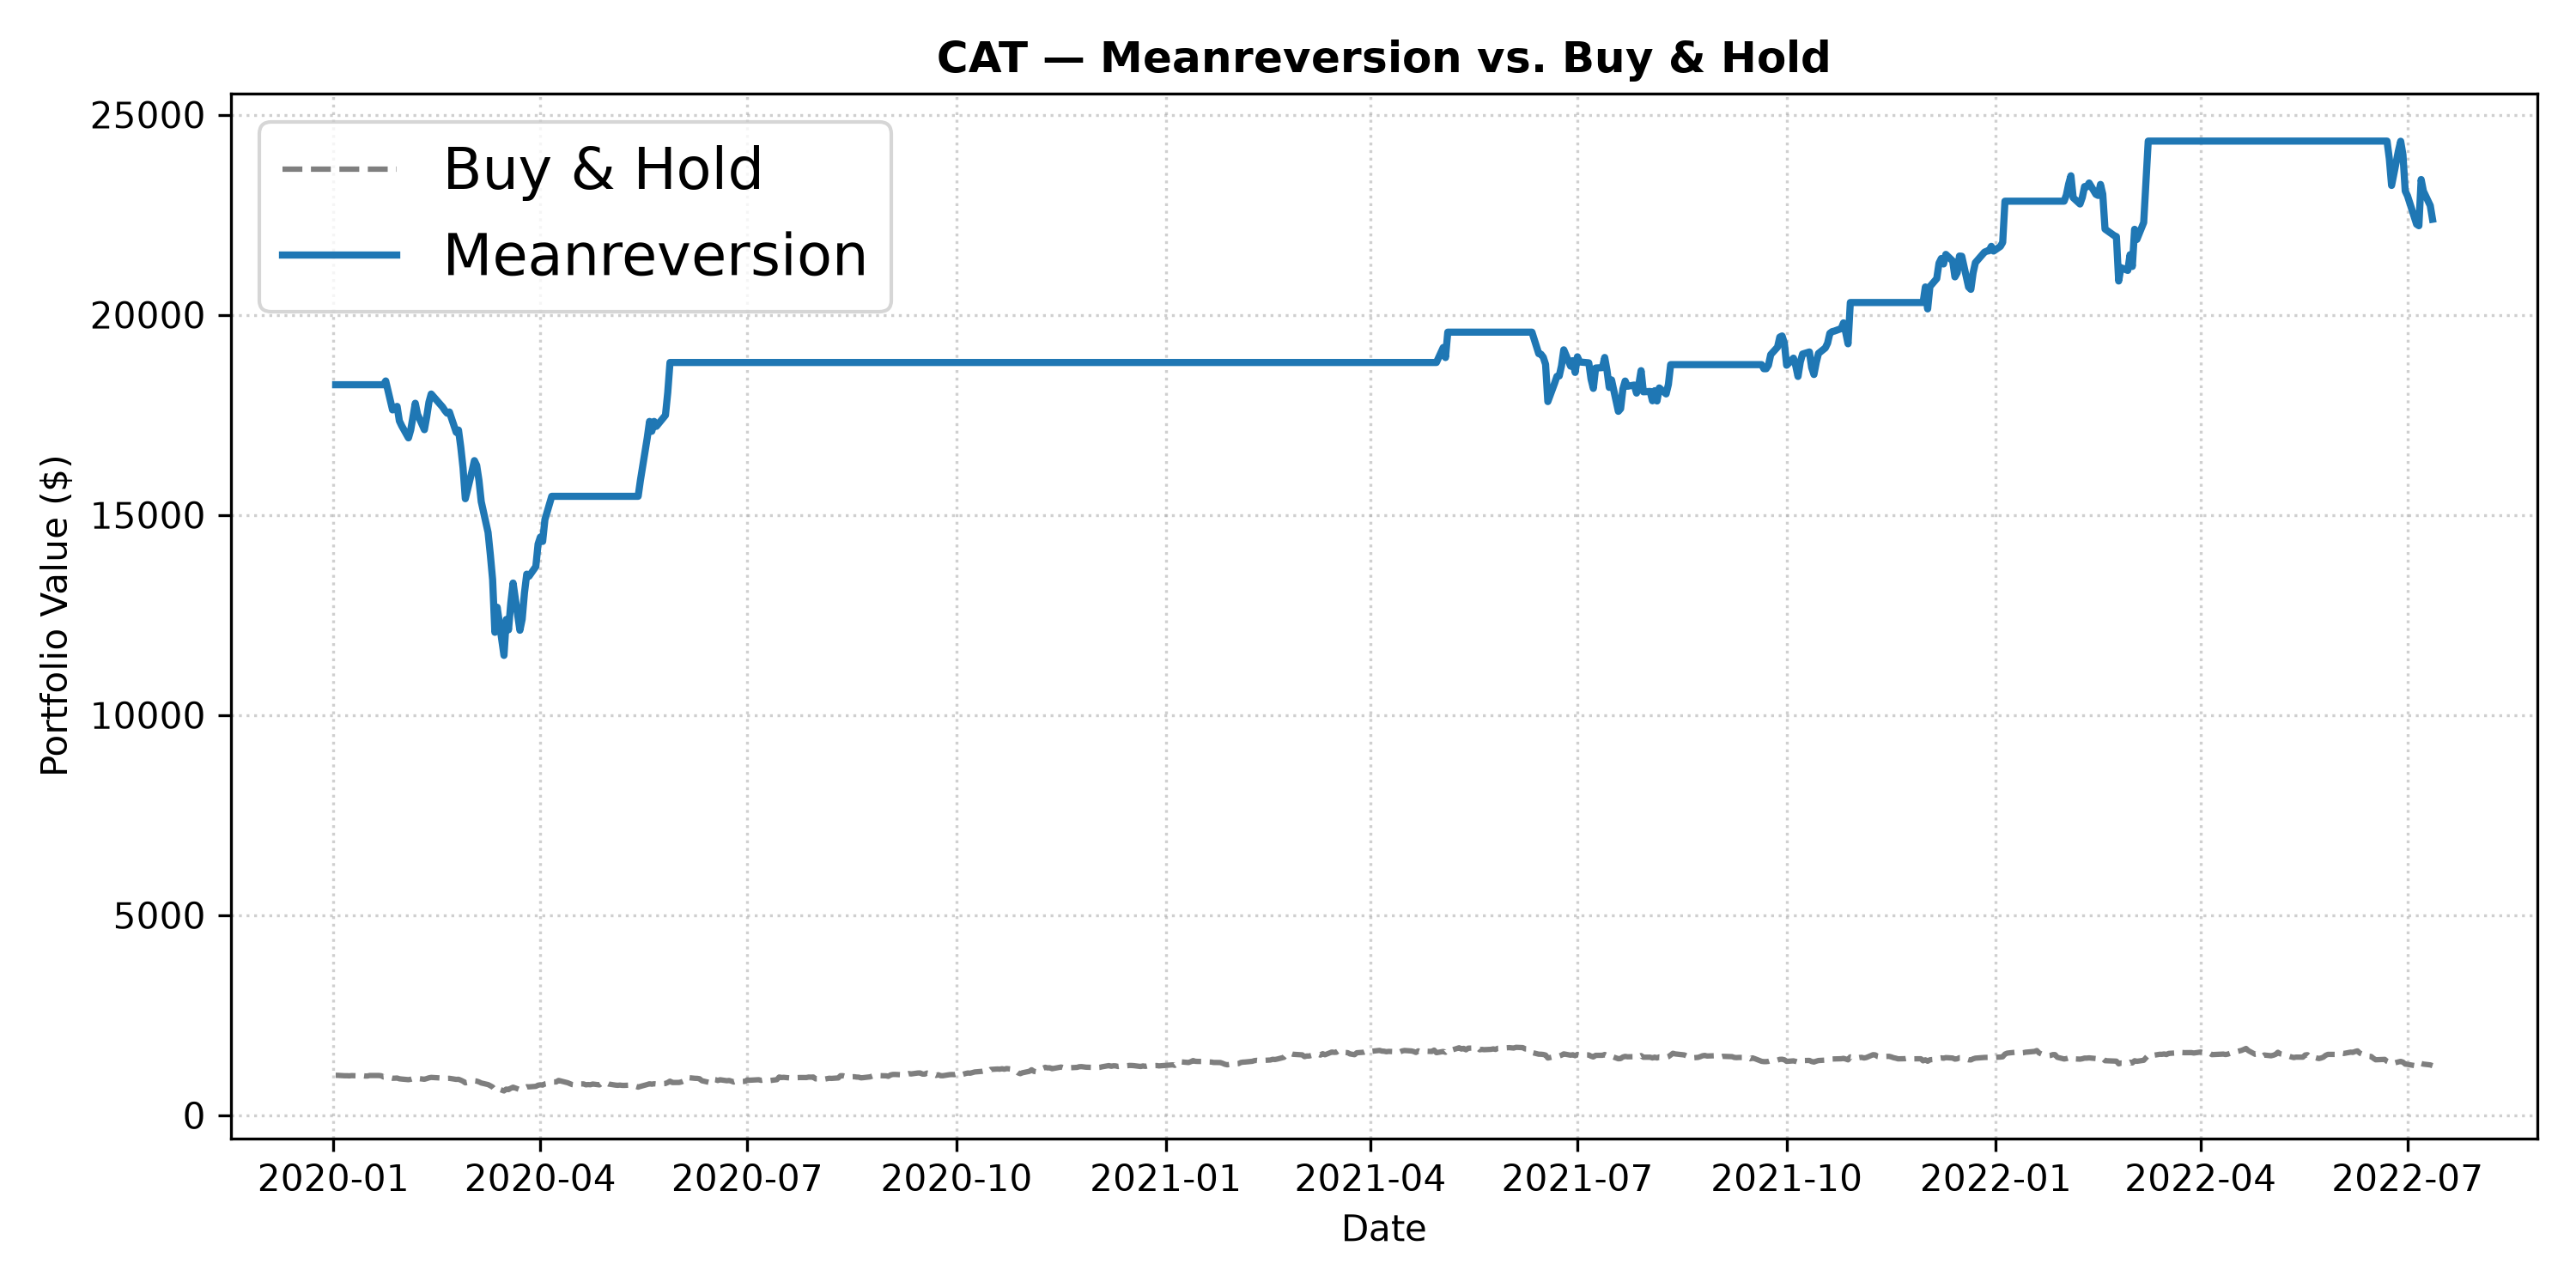
\includegraphics[width=0.85\textwidth]{../results/CAT/CAT_meanreversion_vs_bah.png}
    \caption{Performance comparison on CAT (Cyclical Industrial Sector).}
    \label{fig:meanreversion_cat}
\end{figure}

\begin{figure}[H]
    \centering
    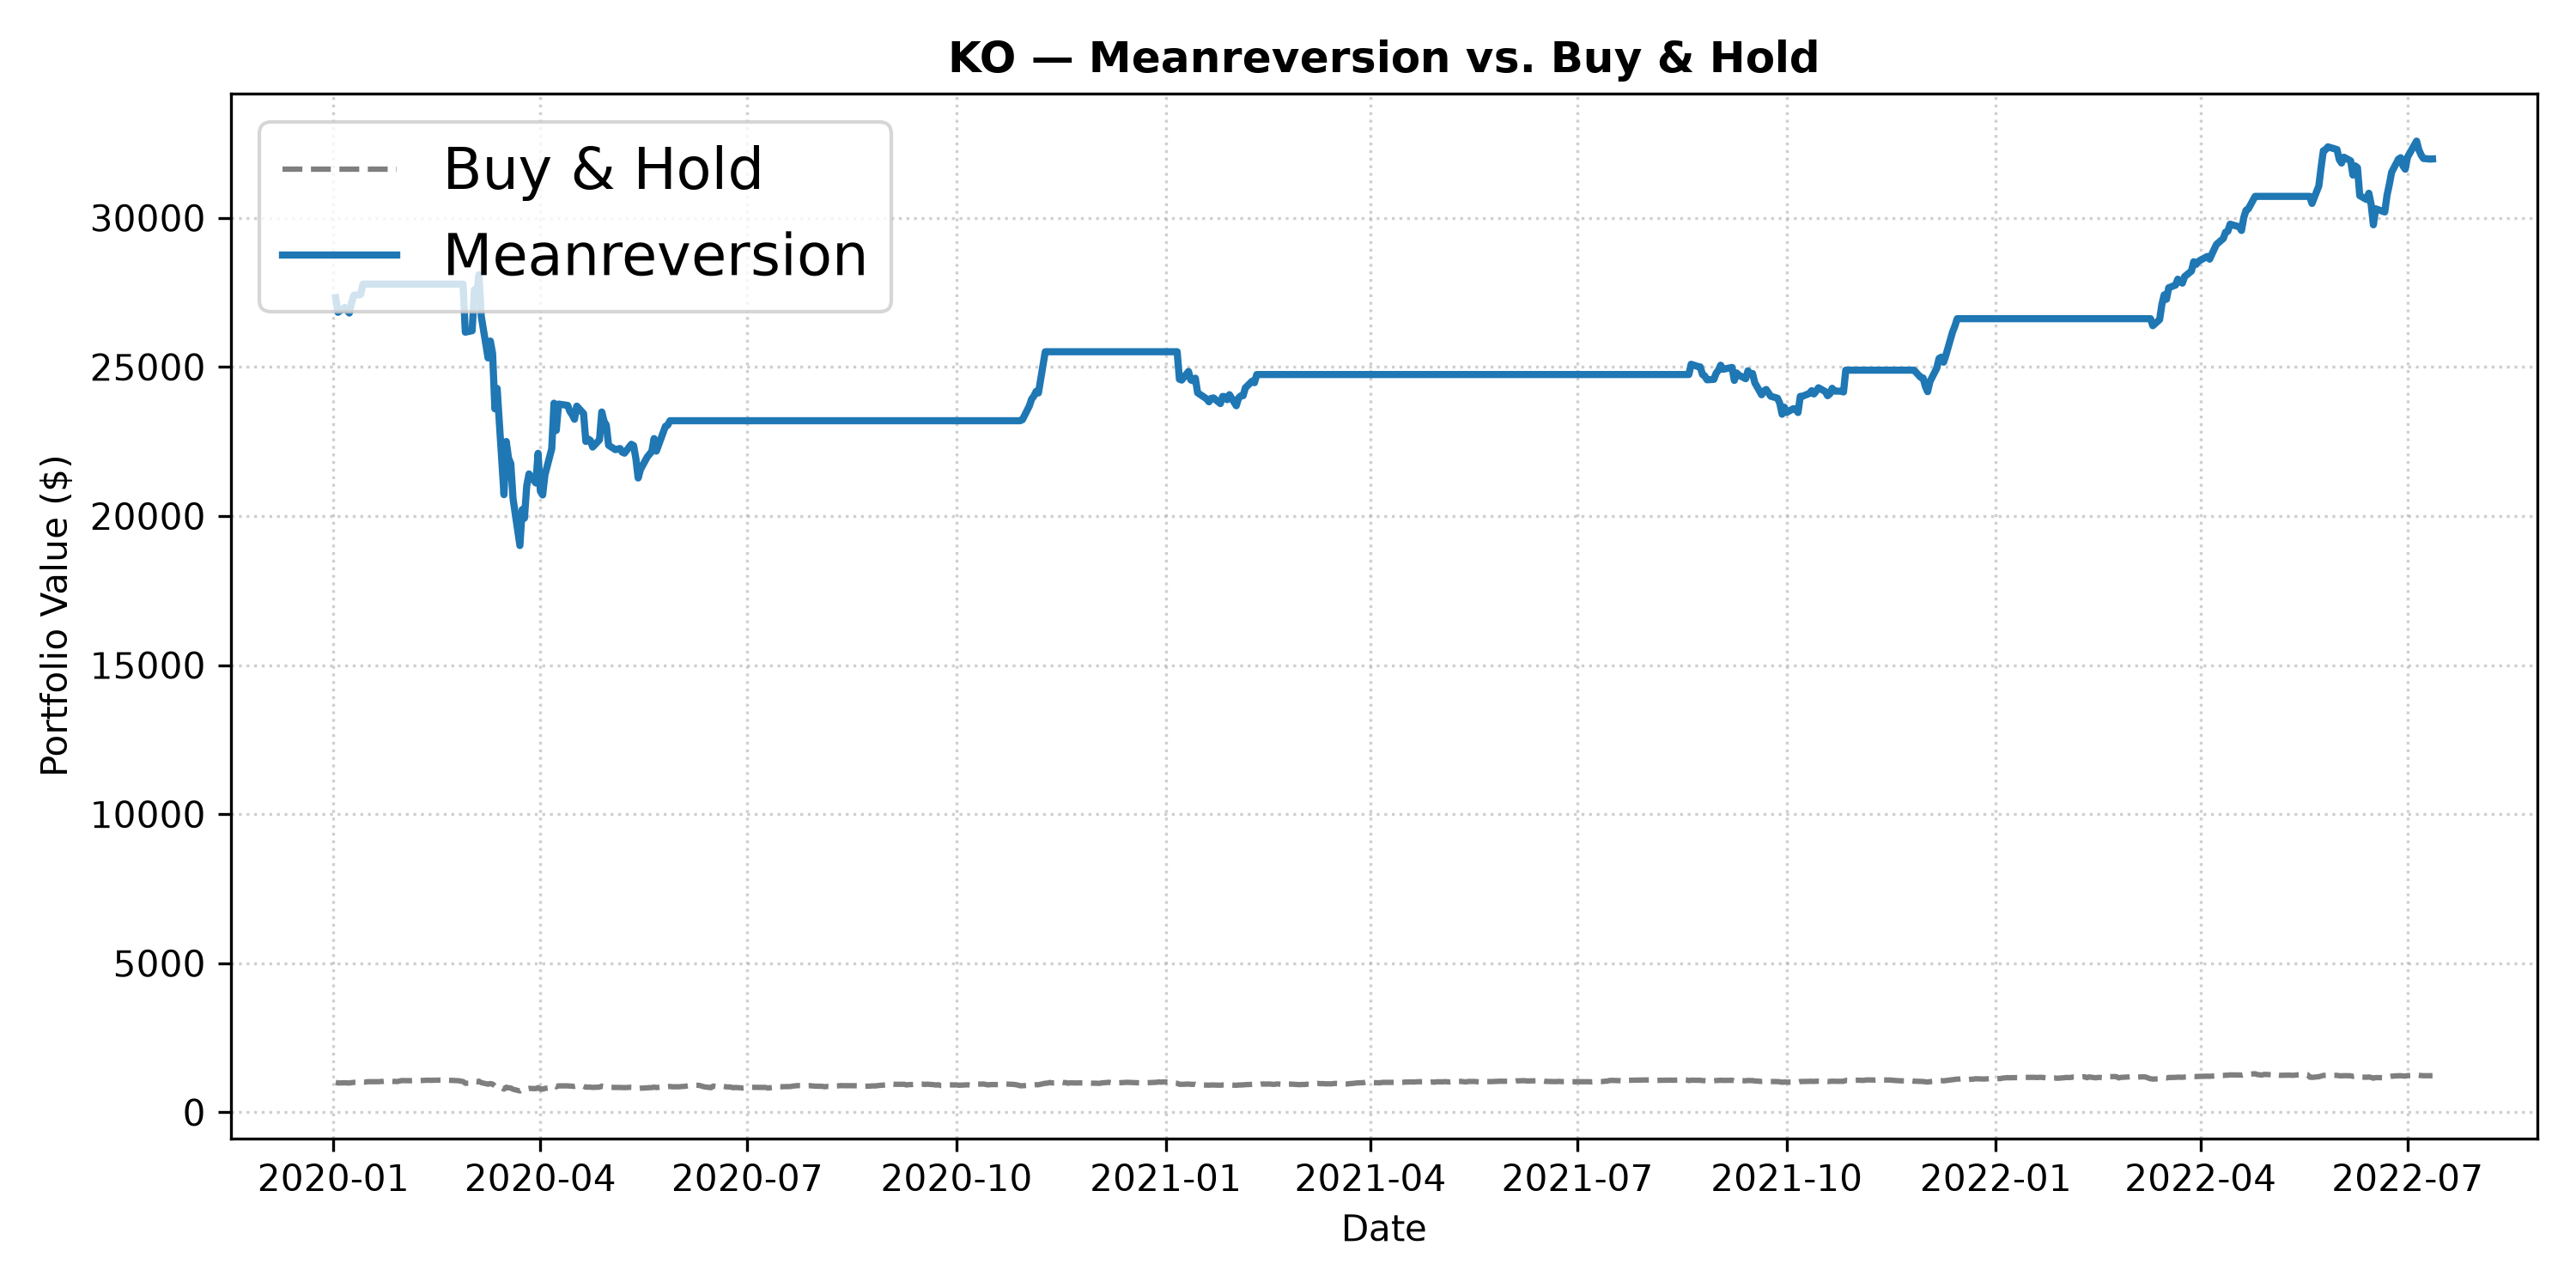
\includegraphics[width=0.85\textwidth]{../results/KO/KO_meanreversion_vs_bah.png}
    \caption{Performance comparison on KO (Defensive Consumer Staples Sector).}
    \label{fig:meanreversion_ko}
\end{figure}

\subsection{XGBoost Performance}
The XGBoost strategy showed moderate and relatively consistent performance on AAPL and CAT. Its performance remained relatively stable throughout the testing period, staying around the middle of the graph. In contrast, the performance on KO was considerably lower. After an initial decline, it remained at a low level for most of the testing period, indicating that the strategy was less effective for KO.

\begin{figure}[H]
    \centering
    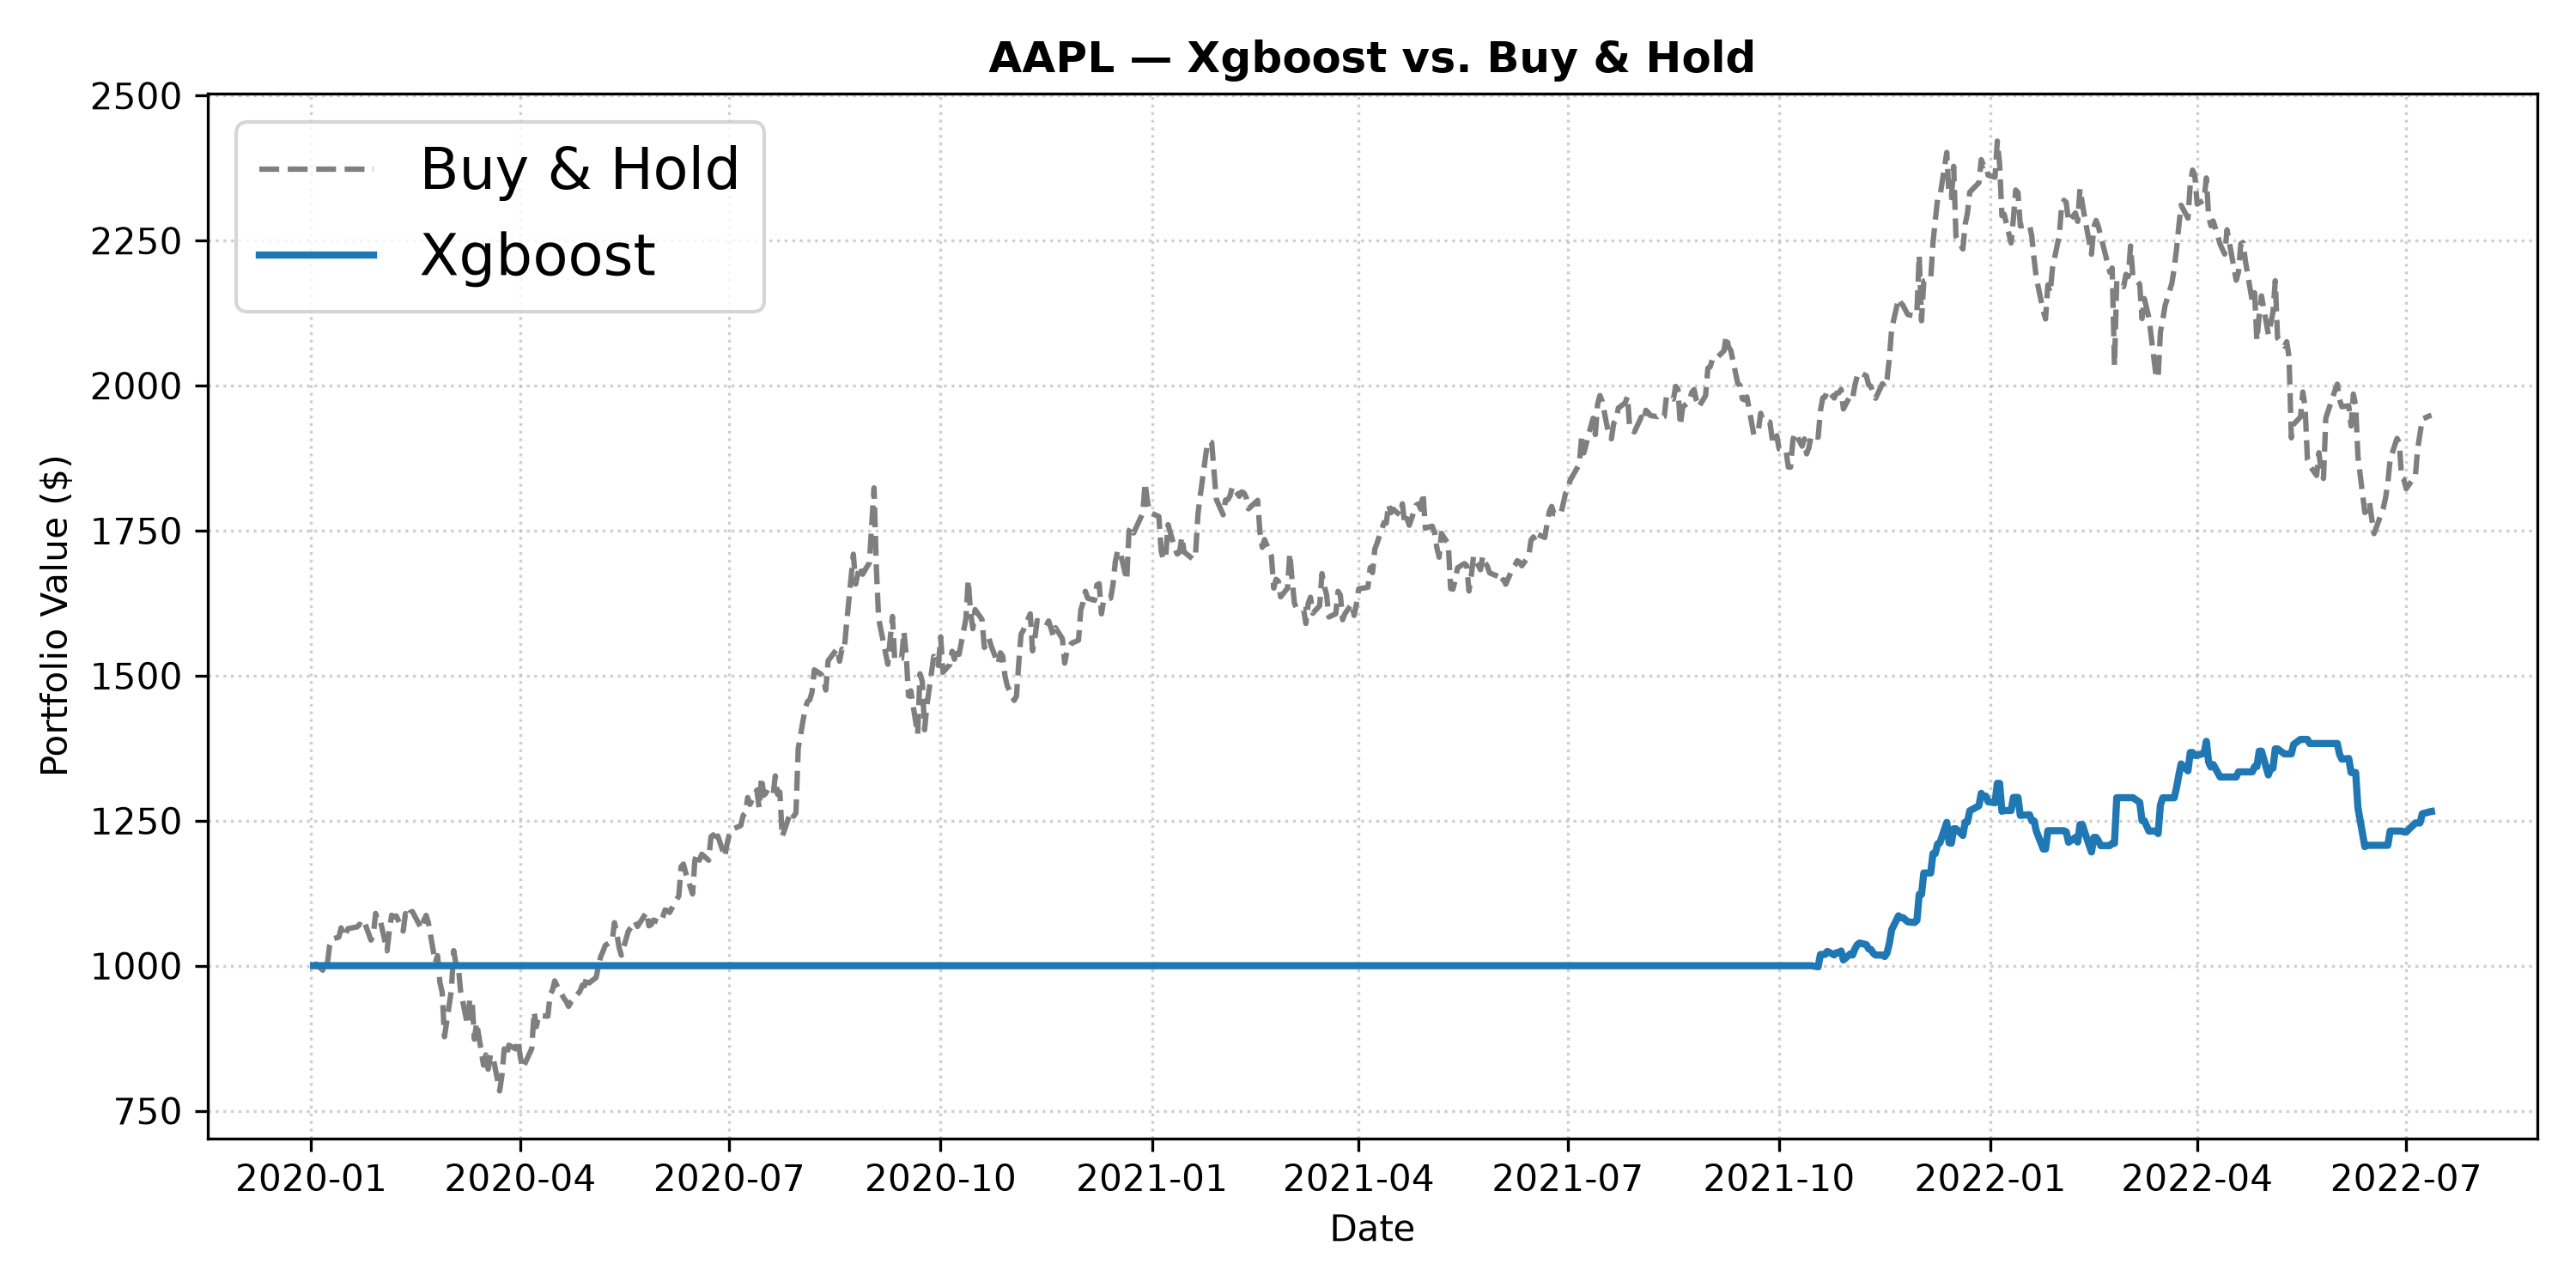
\includegraphics[width=0.85\textwidth]{../results/AAPL/AAPL_xgboost_vs_bah.png}
    \caption{Performance comparison on AAPL (High-Volatility Growth Sector).}
    \label{fig:xgboost_aapl}
\end{figure}

\begin{figure}[H]
    \centering
    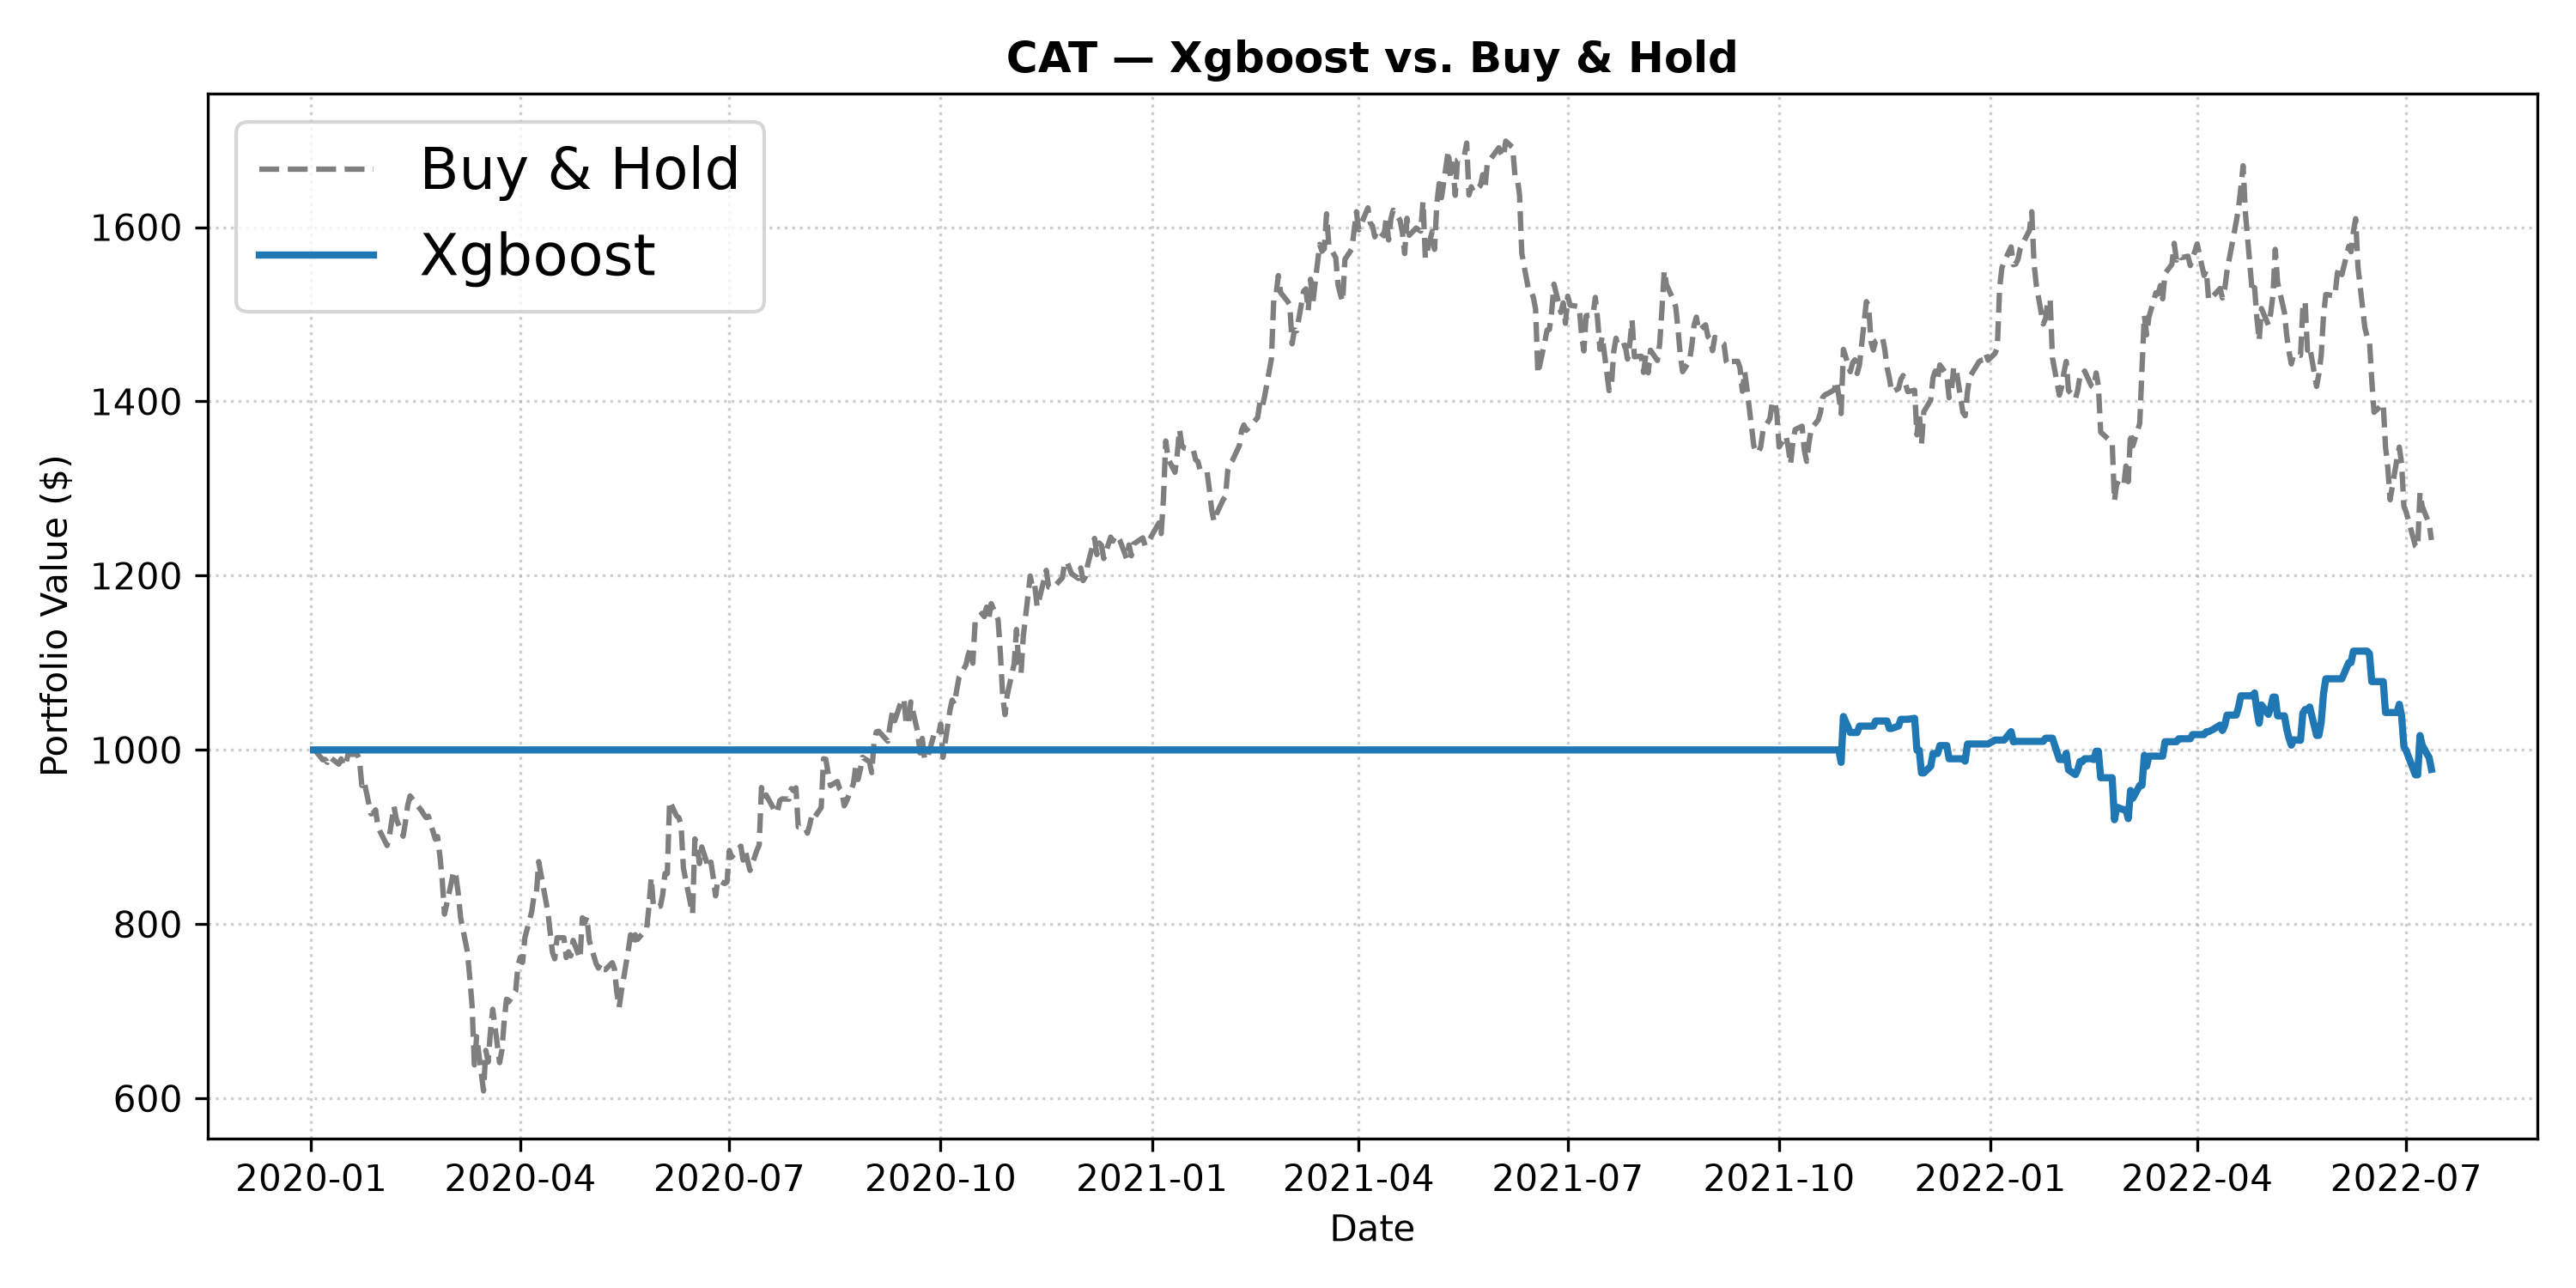
\includegraphics[width=0.85\textwidth]{../results/CAT/CAT_xgboost_vs_bah.png}
    \caption{Performance comparison on CAT (Cyclical Industrial Sector).}
    \label{fig:xgboost_cat}
\end{figure}

\begin{figure}[H]
    \centering
    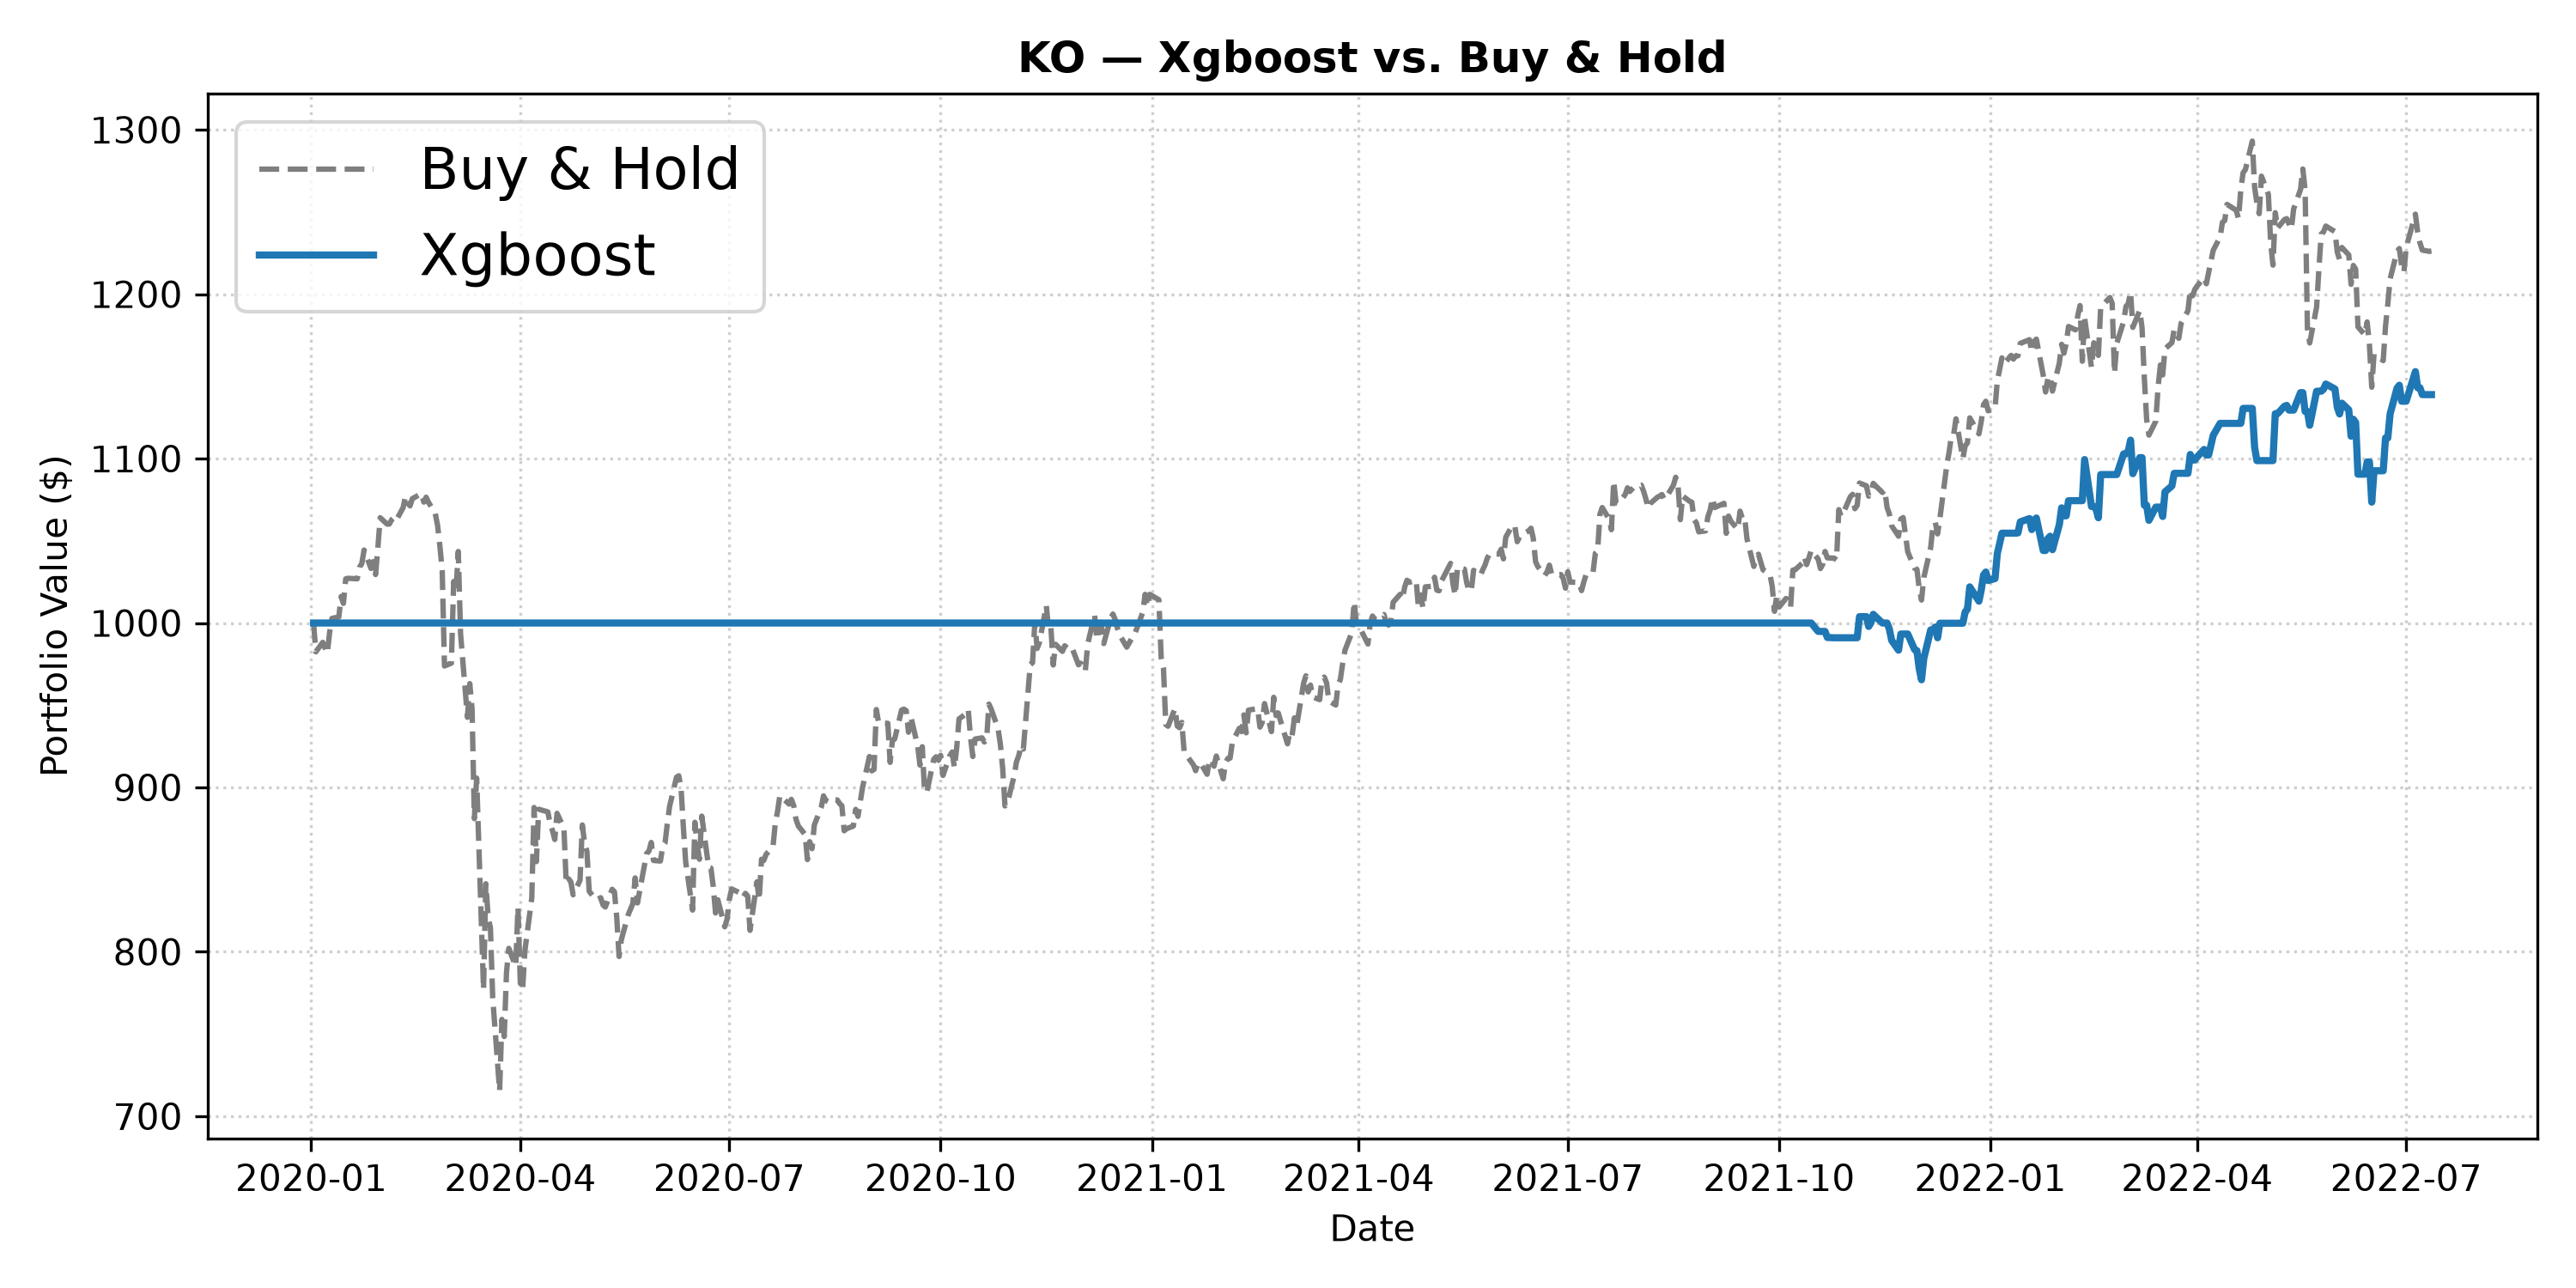
\includegraphics[width=0.85\textwidth]{../results/KO/KO_xgboost_vs_bah.png}
    \caption{Performance comparison on KO (Defensive Consumer Staples Sector).}
    \label{fig:xgboost_ko}
\end{figure}

\FloatBarrier

\subsection{Neural Network Performance}
The multi-layer perceptron neural network strategy displayed mixed performance across sectors, demonstrating sensitivity to signal noise in out-of-sample data.

\begin{figure}[H]
    \centering
    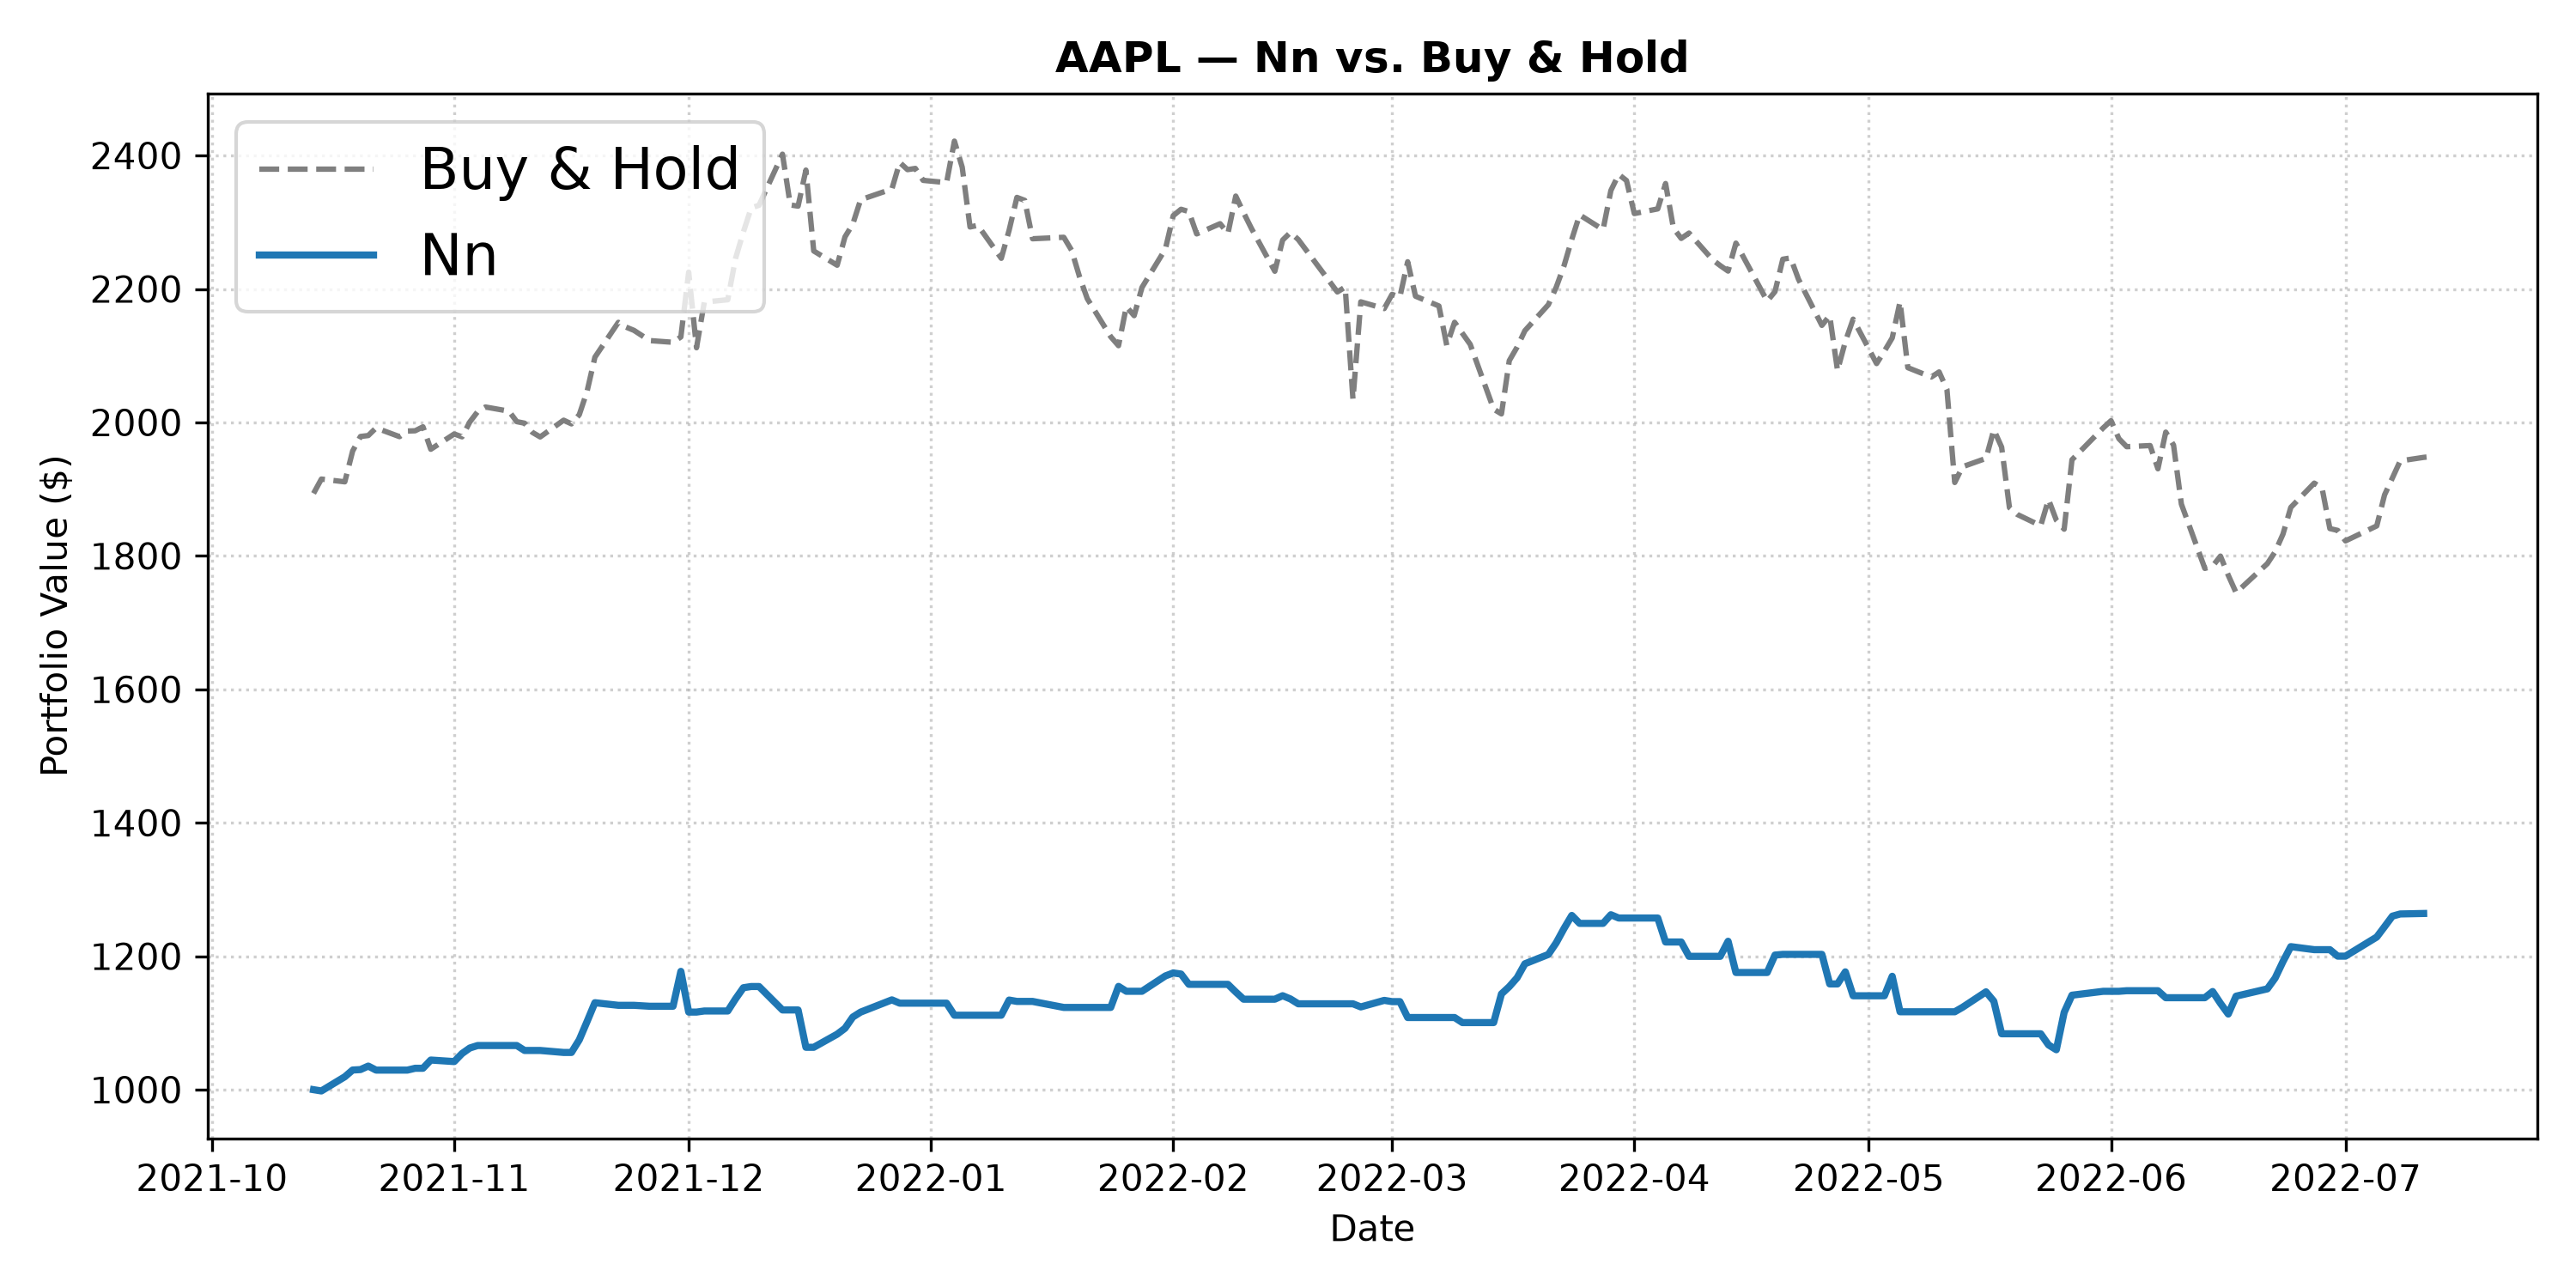
\includegraphics[width=0.85\textwidth]{../results/AAPL/AAPL_nn_vs_bah.png}
    \caption{Performance comparison on AAPL (High-Volatility Growth Sector).}
    \label{fig:nn_aapl}
\end{figure}

\begin{figure}[H]
    \centering
    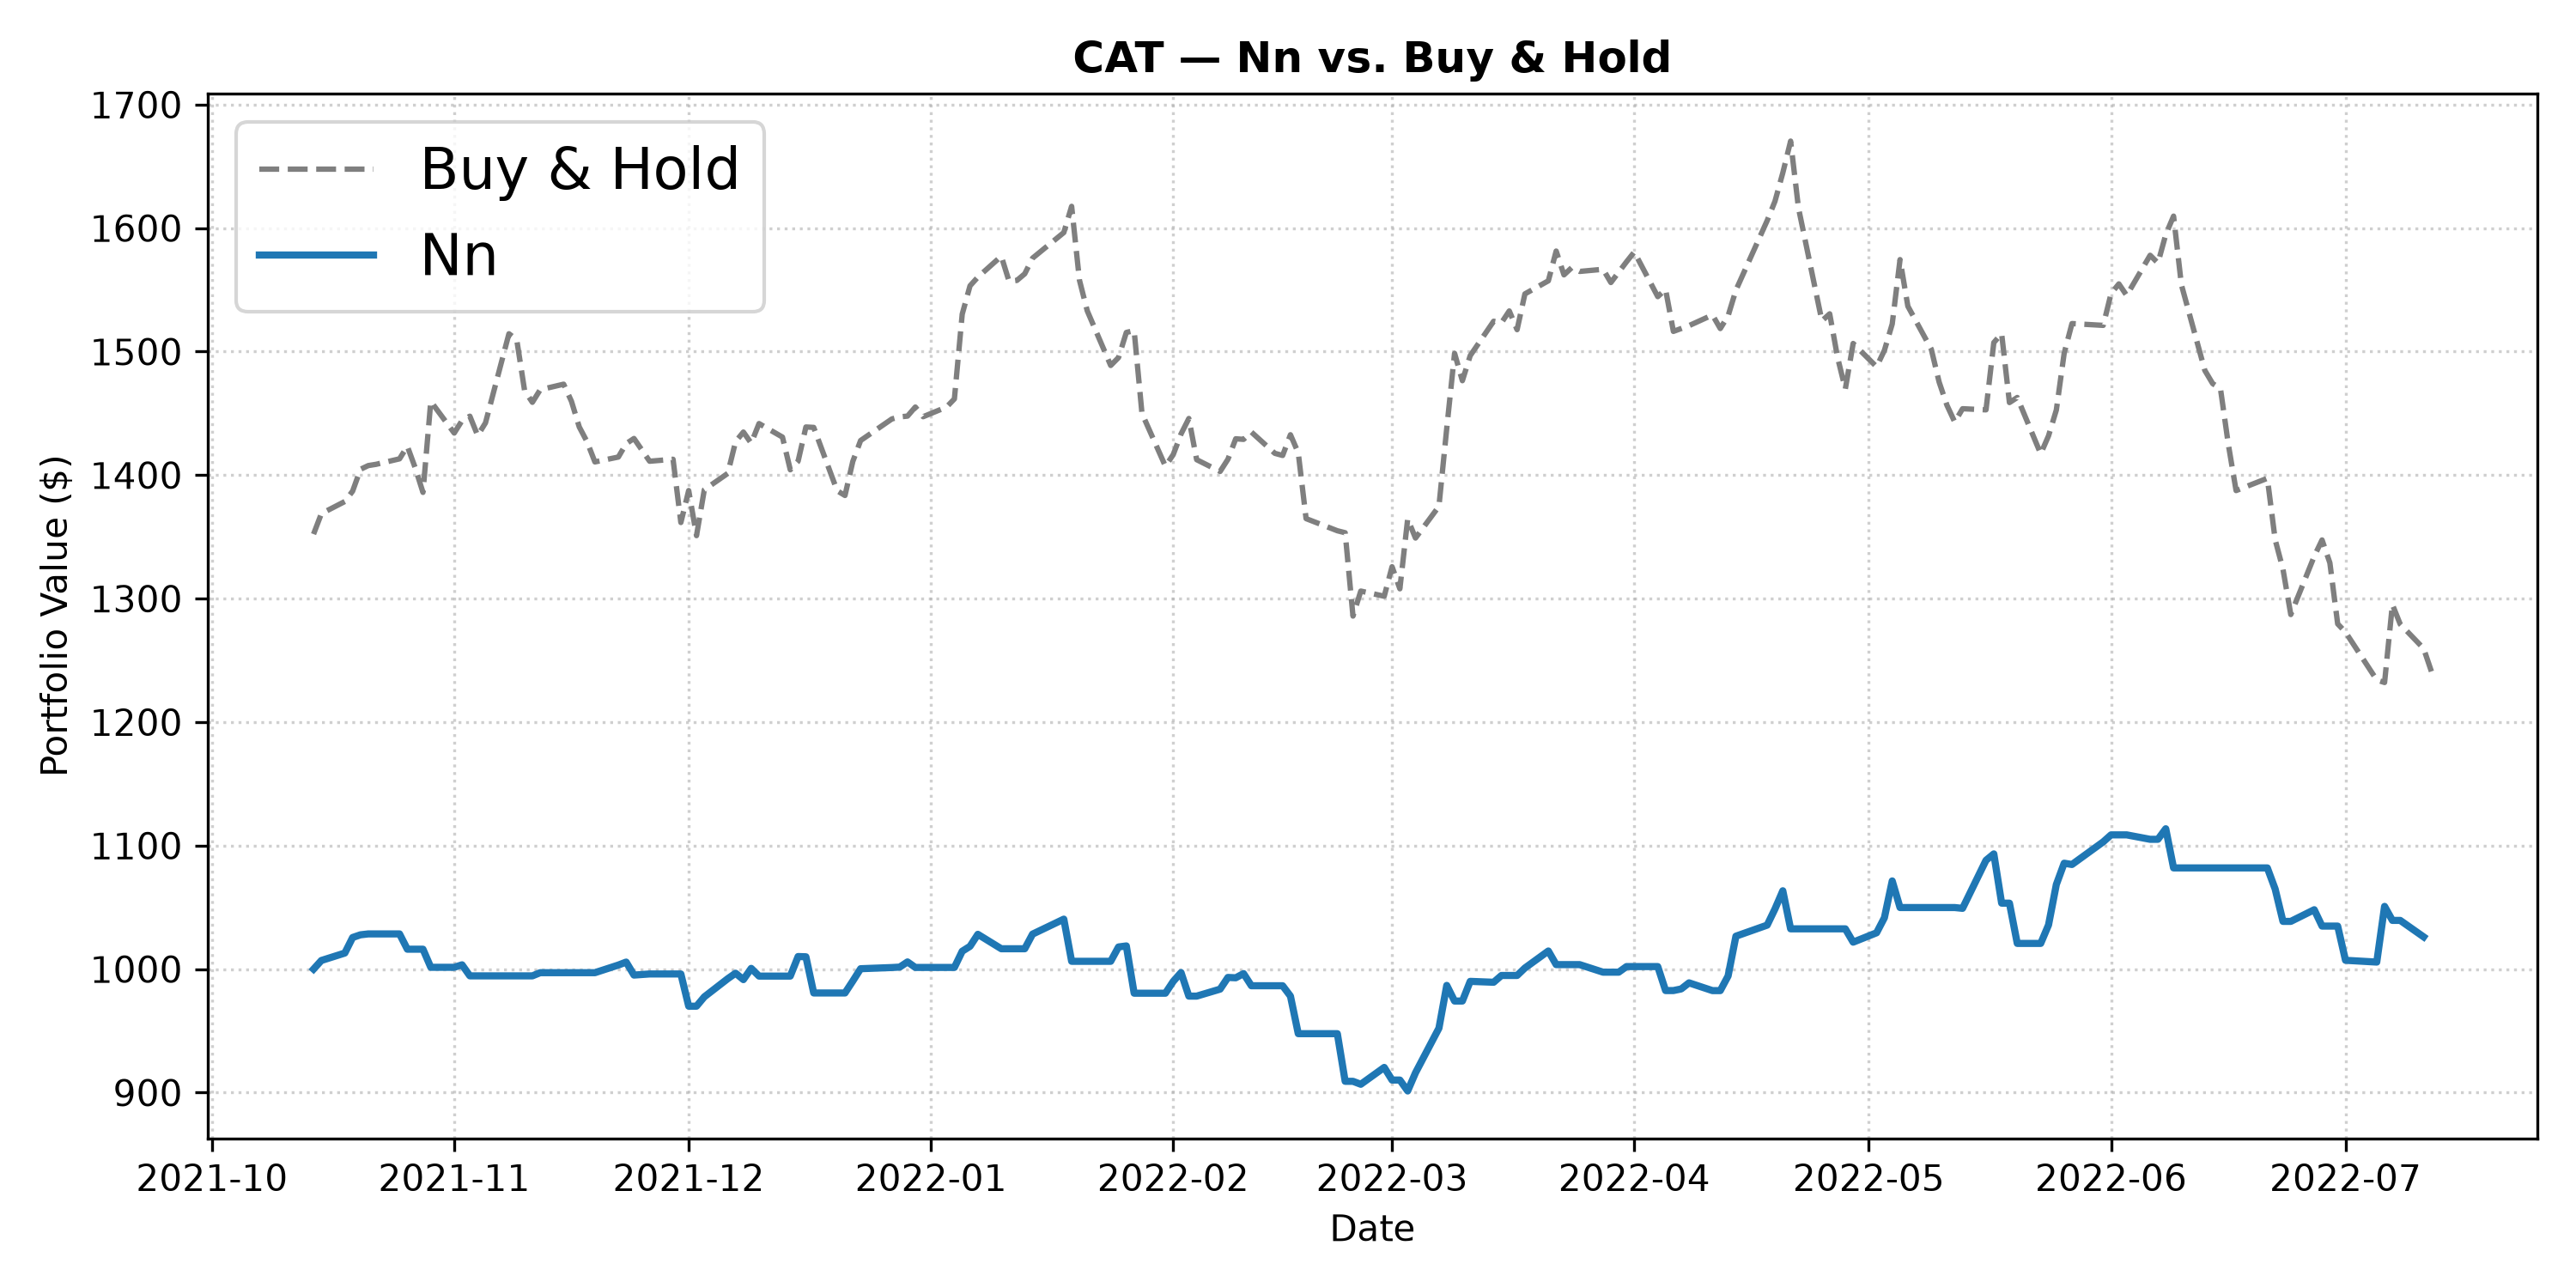
\includegraphics[width=0.85\textwidth]{../results/CAT/CAT_nn_vs_bah.png}
    \caption{Performance comparison on CAT (Cyclical Industrial Sector).}
    \label{fig:nn_cat}
\end{figure}

\begin{figure}[H]
    \centering
    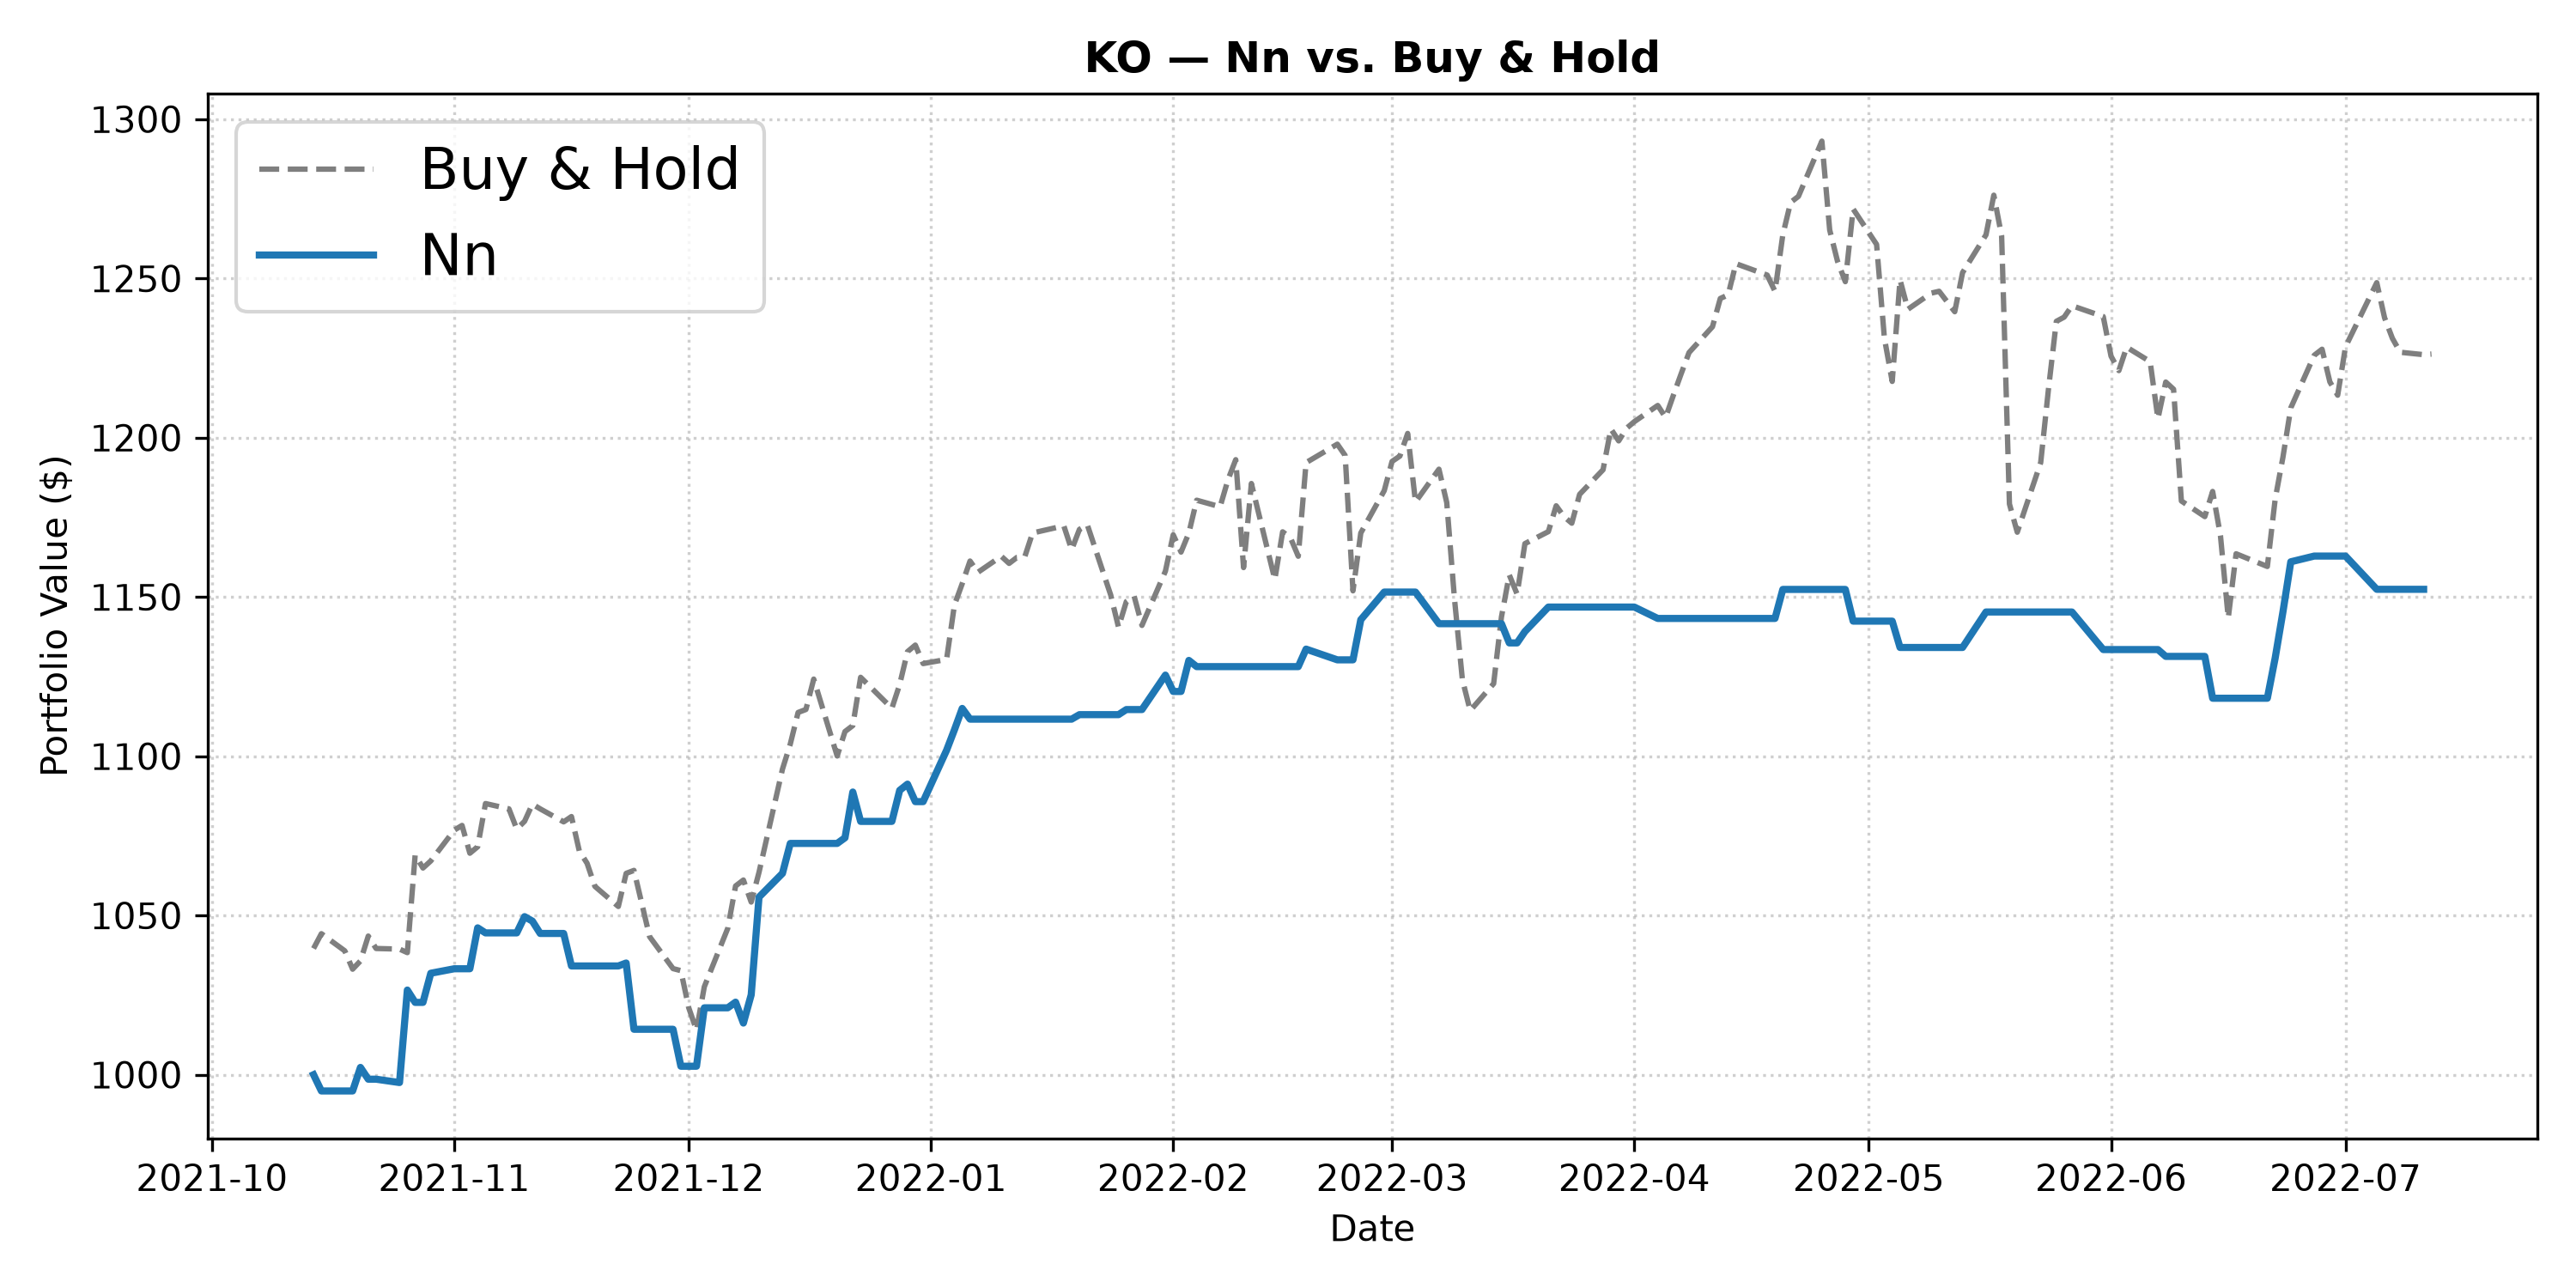
\includegraphics[width=0.85\textwidth]{../results/KO/KO_nn_vs_bah.png}
    \caption{Performance comparison on KO (Defensive Consumer Staples Sector).}
    \label{fig:nn_ko}
\end{figure}

\FloatBarrier

\newpage
\clearpage

\section{Discussion}

\subsection{Interpretation of Results}
\begin{itemize}
    \item \textbf{Rule-Based Benchmarks vs. Complex Models:} Simple trend-following models (Momentum and Moving Average) captured broad directional trends effectively during strong multi-year market expansions.
    \item \textbf{KNN-Filtered Momentum Underperformed:} The \textit{KNN-Filtered Momentum} strategy fell well short of expectations. While the concept sounds promising on paper, adding extra layers of complexity introduces unnecessary friction---causing the model to hold back from buying or selling when the obvious, profitable move was to take the trade.
    \item \textbf{Mean Reversion Inefficiency:} The Standard Deviation Moving Average Mean Reversion strategy suffered from extreme cash drag by enforcing strict deviation thresholds ($V_t \le -T$), missing long-term upside momentum in secularly growing equities.
    \item \textbf{Machine Learning \& Neural Networks:} Tree-based models (XGBoost) and Neural Networks exhibited moderate performance on higher-volatility growth stocks (AAPL, CAT) but underperformed on lower-beta assets (KO), highlighting high vulnerability to out-of-sample distributional shift.
\end{itemize}

\subsection{Hypothesis Testing}
\begin{itemize}
    \item \textbf{$H_0$ (Null Hypothesis):} The algorithmic trading strategies (Momentum, Moving Average, KNN-Filtered Momentum, Mean Reversion, XGBoost, and Neural Network) do not generate statistically significant excess risk-adjusted returns (Sharpe ratio) relative to the Buy \& Hold benchmark.
    \item \textbf{$H_1$ (Alternative Hypothesis):} The systematic trading strategies outperform the Buy \& Hold baseline on a risk-adjusted basis.
    \item \textbf{Outcome:} Based on the backtested portfolio values and risk metrics, simple benchmark strategies often maintained strong performance, whereas higher-complexity models (e.g., KNN-Filtered Momentum) failed to consistently beat Buy \& Hold, leading to a failure to reject $H_0$ across all complex strategies.
\end{itemize}

\subsection{Methodological Limitations}
\begin{itemize}
    \item \textbf{Fixed Asset Universe:} The study evaluated a limited subset of equities (e.g., AAPL, CAT, KO), which may introduce asset-specific behavior that does not generalize across all market conditions or sectors.
    \item \textbf{Backtest Horizon:} Testing over a specific historical window (e.g., starting 2020) exposes the results to regime-specific dynamics such as COVID-19 volatility and market recovery phases.
    \item \textbf{Parameter Fixedness:} Moving average windows ($m$) and hyperparameter choices for machine learning models were fixed rather than dynamically recalibrated via rolling cross-validation.
\end{itemize}

\subsection{Sources of Bias}
\begin{itemize}
    \item \textbf{Look-Ahead Bias:} Ensured $y_t$ signals use information available strictly at time $t$, though signal execution at $Open_{t+1}$ must assume zero execution delay or slippage.
    \item \textbf{Survivorship Bias:} Selecting high-profile, continuously traded equities over the sample period inherently selects historical market winners.
    \item \textbf{Overfitting Risk:} Machine learning strategies like XGBoost, KNN, and Neural Networks risk overfitting to historical feature distributions without guaranteeing out-of-sample stability.
\end{itemize}

\subsection{Future Research Directions}
\begin{itemize}
    \item \textbf{Dynamic Parameter Optimization:} Incorporate rolling walk-forward optimization for parameter selection to adapt to changing volatility regimes.
    \item \textbf{Transaction \& Friction Modeling:} Introduce realistic bid-ask spread friction, market impact costs, and variable order execution delays to evaluate post-cost performance.
    \item \textbf{Expanded Multi-Asset Universe:} Apply the strategies across broader asset classes (e.g., indices, commodities, forex) to evaluate cross-asset robustness.
\end{itemize}

\newpage

\section{Conclusion}

This paper systematically evaluated a diverse suite of quantitative trading algorithms---ranging from classical rule-based indicators to supervised machine learning architectures---against a passive Buy and Hold benchmark across three distinct market equities (AAPL, CAT, and KO).

The empirical results demonstrate that increased algorithmic complexity does not consistently yield superior risk-adjusted returns in uncalibrated settings. Simple trend-following strategies effectively captured structural market movements, whereas complex filtering models like KNN-Filtered Momentum and Neural Networks suffered from trade friction and cash drag. Consequently, passive buy-and-hold investing remains a formidable benchmark against uncalibrated quantitative algorithms during prolonged upward trending regimes.

\newpage

\section{Declaration of AI Assistance}
During the preparation of this paper, ChatGPT and Gemini were used solely for grammatical editing and text polishing. The author created, structured, and formulated all core arguments, concepts, and technical content, and takes full responsibility for the manuscript.

\newpage

\section{References}
\begin{thebibliography}{99}

\bibitem{sp500dataset}
R. Prajapati, ``S\&P 500 Stock Prices Dataset,'' Kaggle Dataset Repository, 2023. [Online]. Available: \texttt{https://www.kaggle.com/datasets/rprkh15/sp500-stock-prices}.

\bibitem{chen2016xgboost}
T. Chen and C. Guestrin, ``XGBoost: A scalable tree boosting system,'' in \textit{Proceedings of the 22nd ACM SIGKDD International Conference on Knowledge Discovery and Data Mining}, 2016, pp. 785--794.

\bibitem{fix1989discriminatory}
E. Fix and J. L. Hodges, ``Discriminatory analysis: Nonparametric discrimination: Consistency properties,'' \textit{International Statistical Review / Revue Internationale de Statistique}, vol. 57, no. 3, pp. 238--247, 1989.

\bibitem{kingma2014adam}
D. P. Kingma and J. Ba, ``Adam: A method for stochastic optimization,'' \textit{arXiv preprint arXiv:1412.6980}, 2014.

\bibitem{loshchilov2017decoupled}
I. Loshchilov and F. Hutter, ``Decoupled weight decay regularization,'' in \textit{International Conference on Learning Representations (ICLR)}, 2019.

\bibitem{sharpe1994sharpe}
W. F. Sharpe, ``The Sharpe ratio,'' \textit{The Journal of Portfolio Management}, vol. 21, no. 1, pp. 49--58, 1994.

\bibitem{paszke2019pytorch}
A. Paszke \textit{et al.}, ``PyTorch: An imperative style, high-performance deep learning library,'' in \textit{Advances in Neural Information Processing Systems (NeurIPS 32)}, 2019, pp. 8024--8035.

\bibitem{pedregosa2011scikit}
F. Pedregosa \textit{et al.}, ``Scikit-learn: Machine learning in Python,'' \textit{Journal of Machine Learning Research}, vol. 12, pp. 2825--2830, 2011.

\bibitem{mckinney2010data}
W. McKinney, ``Data structures for statistical computing in Python,'' in \textit{Proceedings of the 9th Python in Science Conference (SciPy)}, 2010, pp. 56--61.

\end{thebibliography}

\end{document}